\mychapter{Geometria en el pla}{Geometria en el pla}{\begin{center}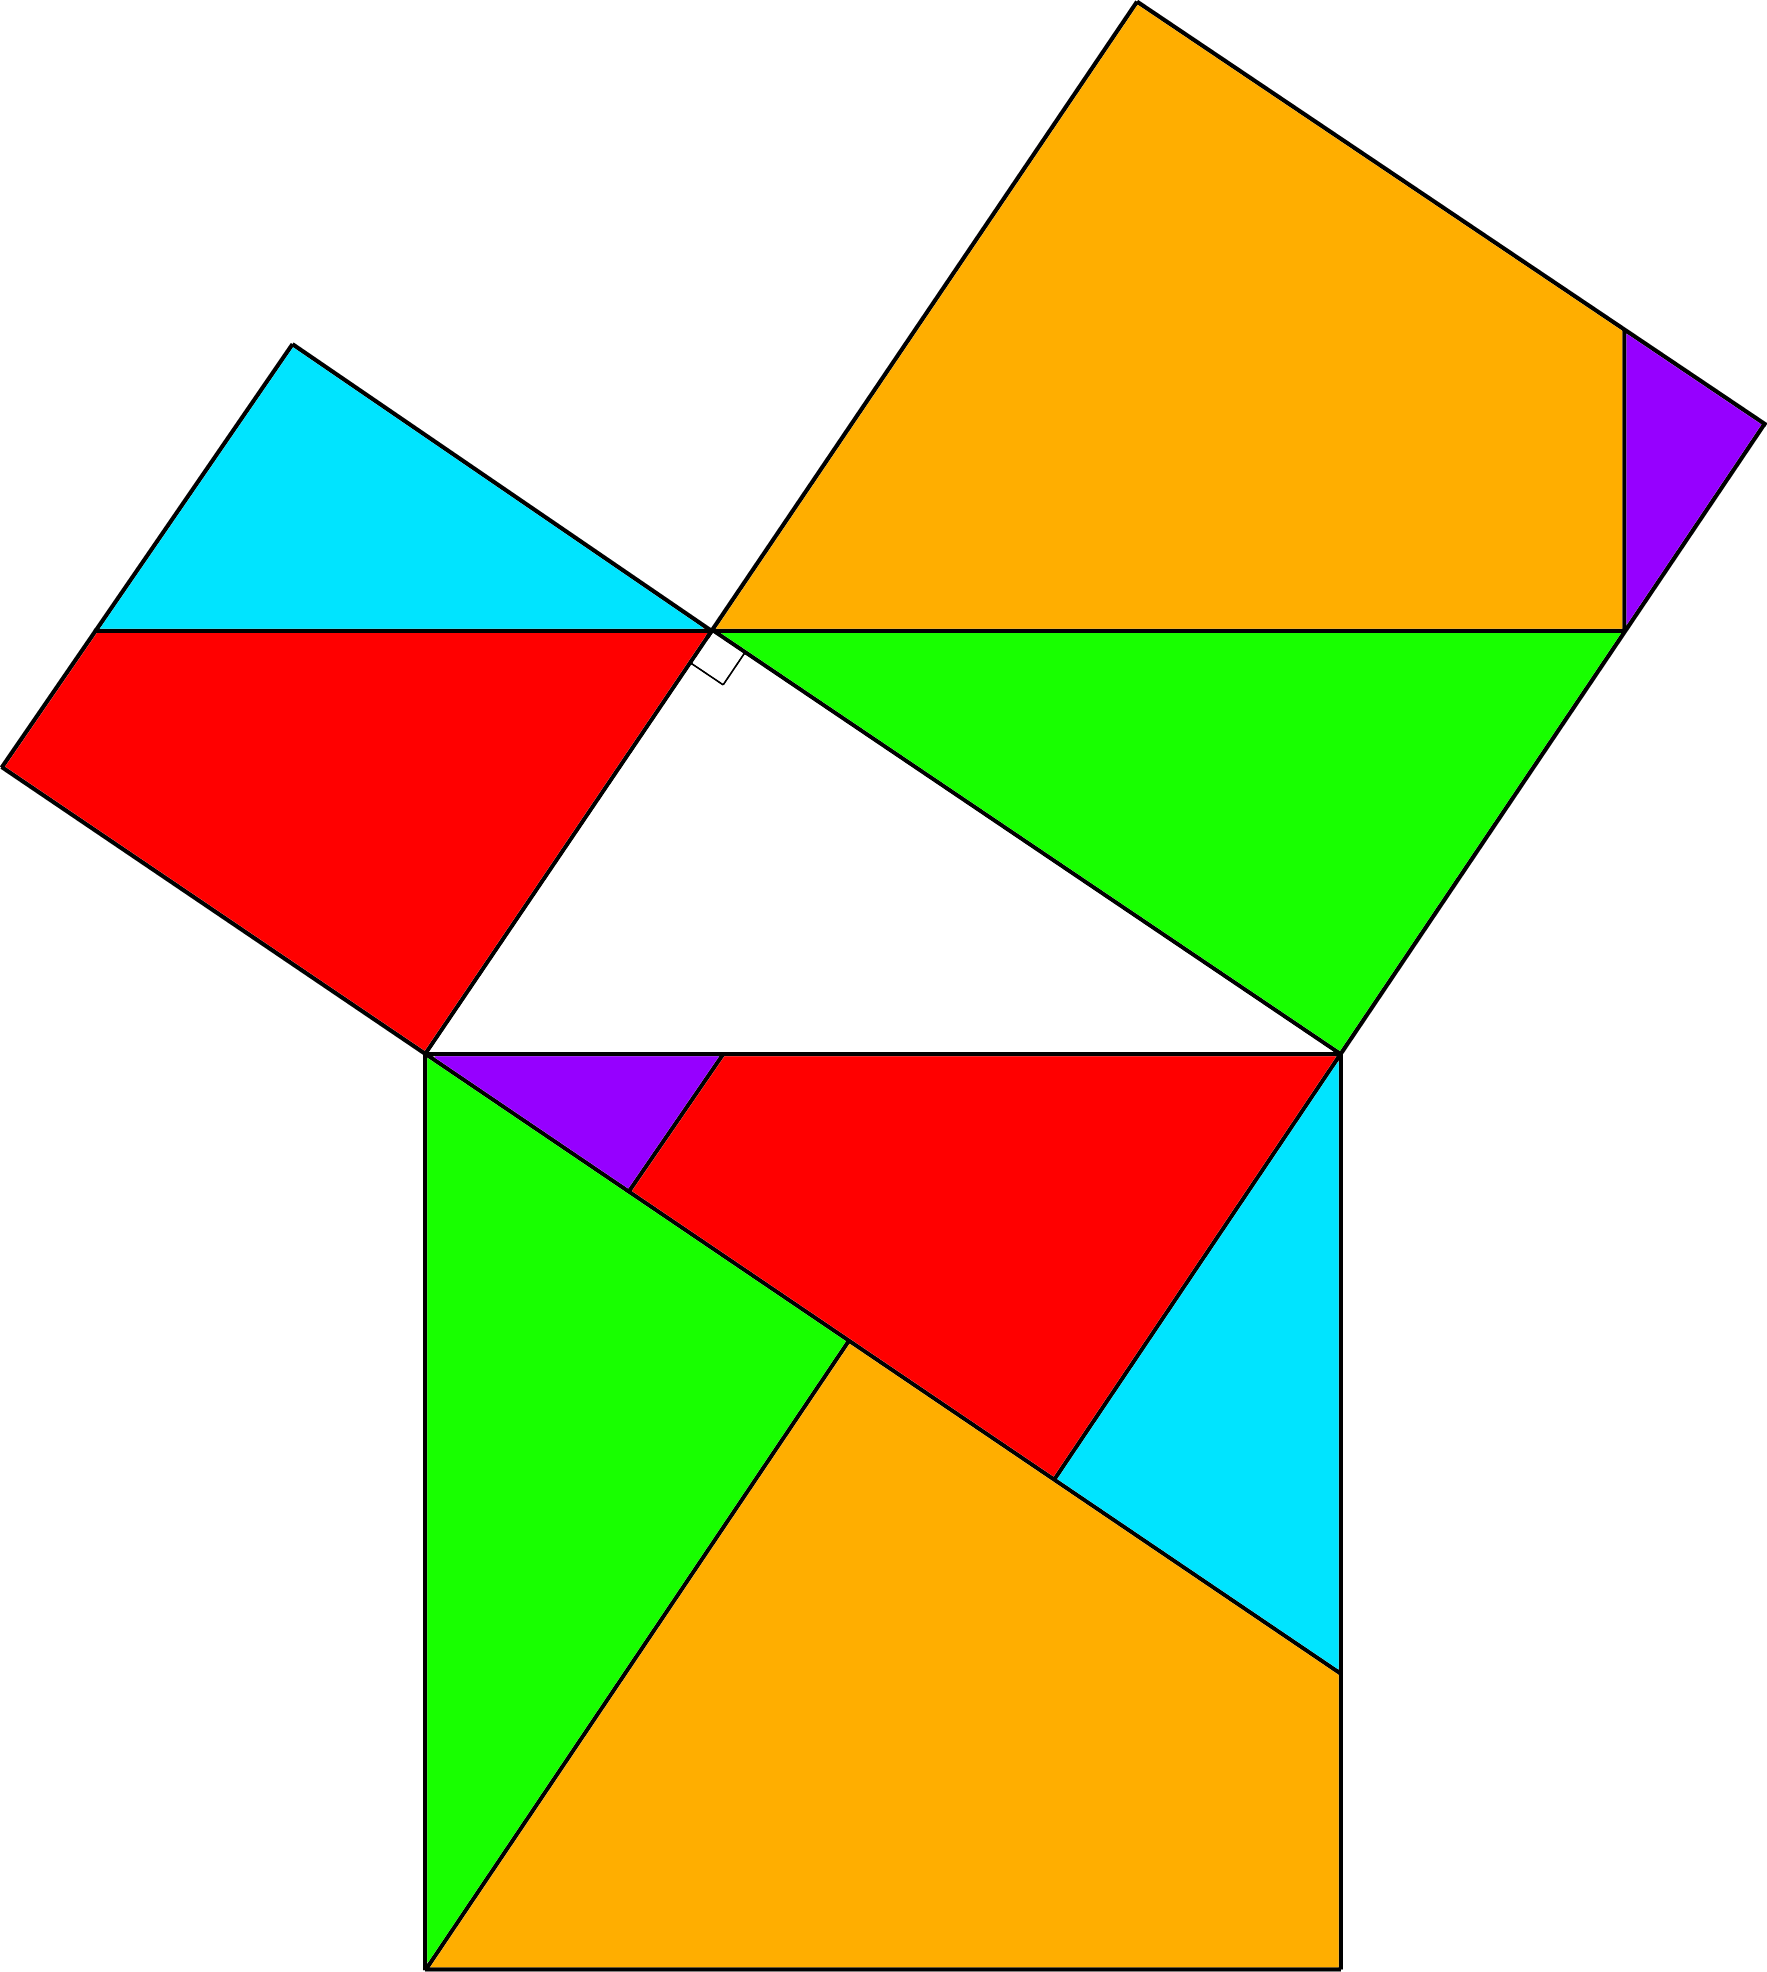
\includegraphics[width=0.9\textwidth]{img-09/pitagoras} \footnotesize Demostració del teorema de Pitàgores\end{center}}{chap:geo2d}

\begin{iniaval}
	
    \begin{minipage}{0.6\textwidth}
			Hem anat a la copisteria i hem fet una fotocòpia ampliada del logo del nostre centre.
			
			\begin{tasks}
			 \task Quina ampliació ens han fet?
			 \task Què valdran les mesures que falten?
			 \task Què val l'àrea del cercle ampliat?
			 \end{tasks}
	\end{minipage}
	\begin{minipage}{0.4\textwidth}
		\centering
			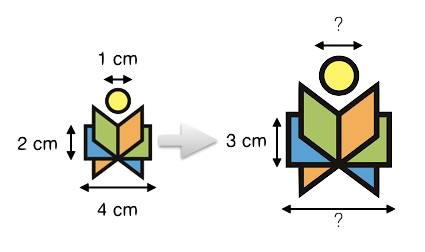
\includegraphics[width=\textwidth]{img-09/ampliacio1}
	\end{minipage}
	 
	 \vso\vso
	
	 \begin{minipage}{0.65\textwidth}
	  d) A casa, estam dissenyant un logo similar amb les mides que apareixen en la figura. Ens agradaria saber quina quantitat de cartolina necessitam per poder fer la figura.  Ens ajudes?

	 \end{minipage}
	 \begin{minipage}{0.35\textwidth}
	 	\centering
	 	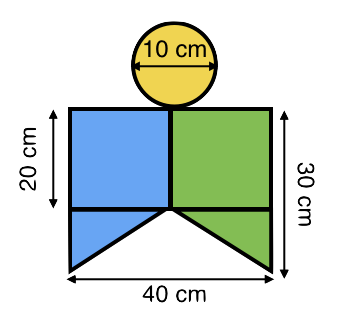
\includegraphics[width=0.9\textwidth]{img-09/ampliacio2}
	 \end{minipage}
	 \vsoo
	 
	 \addanswersline[cols=1]{Avaluació inicial}{0}{[La raó és $r=\dfrac{3}{2}=1.5$. Han ampliat un 150 \%, Les mesures són 1.5 cm i 6 cm, L'àrea del cercle ampliat és 7.1 cm$^2$, $A=1079$ cm$^2$.]}
\end{iniaval}

\newpage
\section{Semblança}

\begin{theorybox}
	\begin{wrapfigure}{R}{0.3\textwidth}
		\centering
			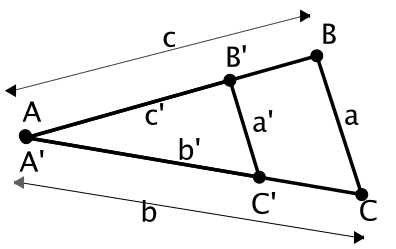
\includegraphics[width=0.28\textwidth]{img-09/trig-semblant}
	\end{wrapfigure}
	
	Dues figures són semblants si són una còpia ampliada o reduïda una de l'altre (sense deformar-la). 
	
	Dues figures semblants \textbf{conserven tots els angles}. Els seus costats són tots proporcionals i la constant de proporcionalitat s'anomena \textbf{raó de la semblança} $r$.
	
	\textbf{Teorema de Tales}: Dos triangles $ABC$ i $A'B'C'$ són semblants si: 
	
	\begin{itemize}
		\item Té dos angles iguals $\hat A = \hat A'$  i $\hat B = \hat B'$ o
		\item Els seus costats són proporcionals $\frac{a}{a'}=\frac{b}{b'}=\frac{c}{c'}=r$
	\end{itemize}
	

\end{theorybox}

\begin{mylist}
\exer  Indica si són semblants els següents parells de triangles:



\begin{tasks}
	\task  Un angle de 80${}^\circ$  i un altre de 40${}^\circ$ . Un angle de 80${}^\circ$  i un altre de 60${}^\circ$ . 
	\task  Triangle isòsceles amb angle desigual de 70${}^\circ$ . Triangle isòsceles amb angle igual de 50${}^\circ$ .
	\task  \textit{A =} 30${}^\circ$ , \textit{b} = 7 cm, \textit{c} = 9 cm. \textit{A'}= 30${}^\circ$ , \textit{b}' = 3.5 cm, \textit{c}' = 4.5 cm
	\task  \textit{a =} 4 cm, \textit{b} = 5 cm, \textit{c} = 7 cm. \textit{a'} = 10 cm, \textit{b'} = 12.5 cm, \textit{c'} = 24.5 cm
\end{tasks}

\answers[cols=1]{[Sí perquè tenen tots els angles iguals, 
	No perquè els seus angles respectius són 70; 55; 55 i 80; 50; 50,
 	Si perquè tenen un angle igual i els costats que els formen són proporcionals (la meitat).
	No perquè $\dfrac{a'}{a} = \dfrac{b'}{b} = 2.5$ però $\dfrac{c'}{c} = 3.5$]}


\exer  Calcula el valor desconegut perquè els triangles siguin semblants:

\begin{tasks}
	\task  \textit{a =} 9 cm, \textit{b} = 6 cm, \textit{c} = 12 cm. \textit{a}' = 6 cm, \textit{b'} = 4 cm, \textit{c'=}?
	\task  \textit{A =} 45${}^\circ$ , \textit{b} = 8 cm, c = 4 cm. \textit{A'} = 45${}^\circ$ , \textit{b'} = 8 cm, \textit{a'=}?
\end{tasks}

\answers{[$c'=8$ cm, $c'=8$ cm]}

\exer  Na Maria mesura 160~cm i la seva ombra mesura 90~cm. En aquest mateix instant es mesura l'ombra d'un edifici i mesura 7,2~m. Quant mesura l'edifici?

\answers{L'edifici mesura 12.8 m.}

\exer  Un triangle té costats de 6 cm, 7 cm i 7 cm. Un triangle semblant a ell té un perímetre de 60 cm. Quant mesuren els seus costats?

\answers{Primer trobam la raó de semblança $\dfrac{60}{(6+7+7)}=3$. Els nous costats s'obtenen de multiplicar per 3 els originals: 18 cm, 21 cm i 21 cm}

\begin{resolt}[E]{
	Calcula $\overline{CD}$ i $\overline{BC}$ de la figura:
	
	\begin{center}
		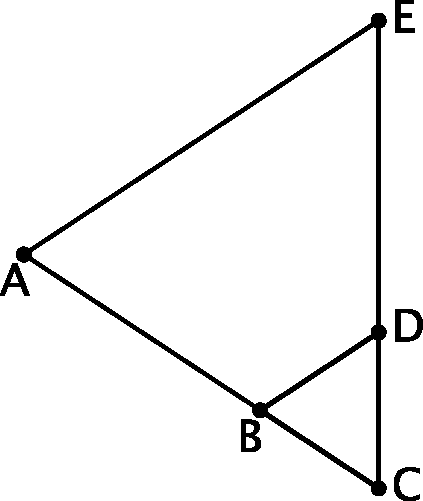
\includegraphics[width=0.2\textwidth]{img-09/sampleTales}
	\end{center}	

sabent que  $\overline{AC}=15$ cm, $\overline{CE}=11$ cm, $\overline{BD}=6.4$ cm i $\overline{AE}=18$ cm.
}
		
		Aplicam que els triangles $\widehat{ACE}$ i $\widehat{BCD}$ són semblants i, per tant, tots els seus costats són proporcionals.
		
		\[ \frac{18}{6.4} = \frac{11}{\overline{CD}}  \quad \rightarrow \quad \overline{CD} = \frac{6.4 \cdot 11}{18} = 3.9 \text{ cm } \]
		
		\quad i
		
		
		\[ \frac{15}{\overline{BC}} = \frac{11}{\overline{3.9}}  \quad \rightarrow \quad \overline{BC} = \frac{15 \cdot 3.9}{11} = 5.3 \text{ cm } \]
\end{resolt}
\newpage

\exer[1]  Calcula els valors de  $x$ i $y$ en les següents figures. 

\begin{tasks}(2)
	\task   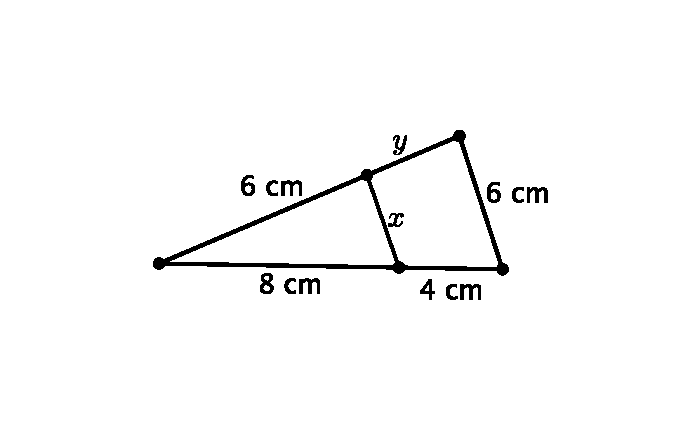
\includegraphics[width=0.3\textwidth]{img-09/trig-semblant2}
	\task    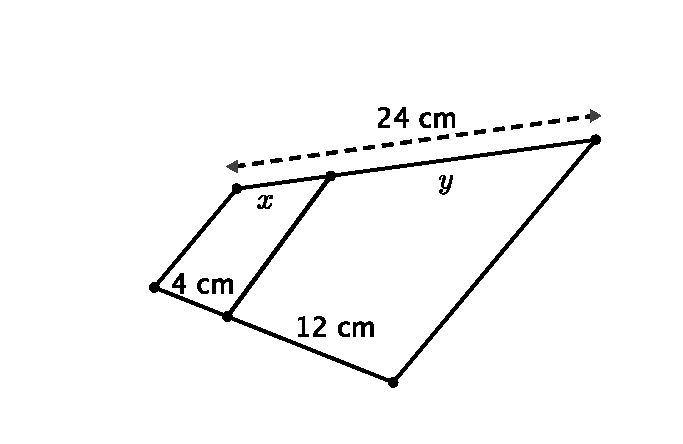
\includegraphics[width=0.35\textwidth]{img-09/trig-semblant5}
\end{tasks}
\answers[cols=1]{[$x=4$ i $y=3$ cm, $x=6$ i $y=18$ cm]}

\exer  Un pal alt es subjecta amb cables d'acer que van del seu extrem superior al sòl. La distància de l'ancoratge d'un dels cables a la base del pal és 6 metres. Posem una barra de 120 centímetres de manera que està perpendicular al sòl i just toca el sòl i el cable. La seva distància a l'ancoratge del cable és 90 centímetres. Calcula la longitud del pal i la longitud del cable d'acer.

 \answers{Esquema:\par 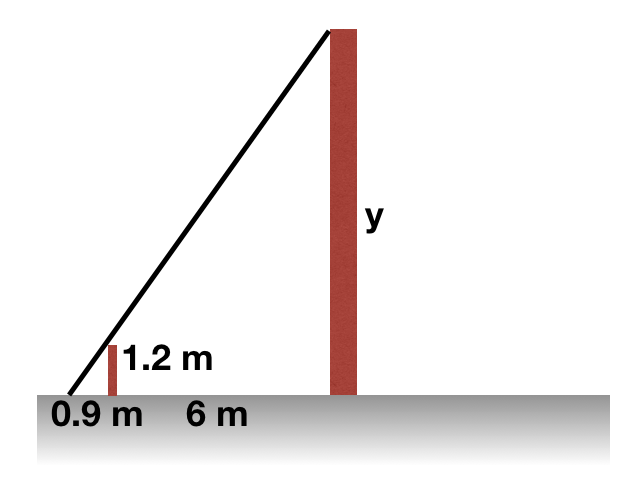
\includegraphics[width=0.3\textwidth]{img-sol/t9-5}\par El pal mesura   8 m i el cable 10 m.}

\exer  Calcula les longituds que s'indiquen:
\begin{tasks}(2)
	\task    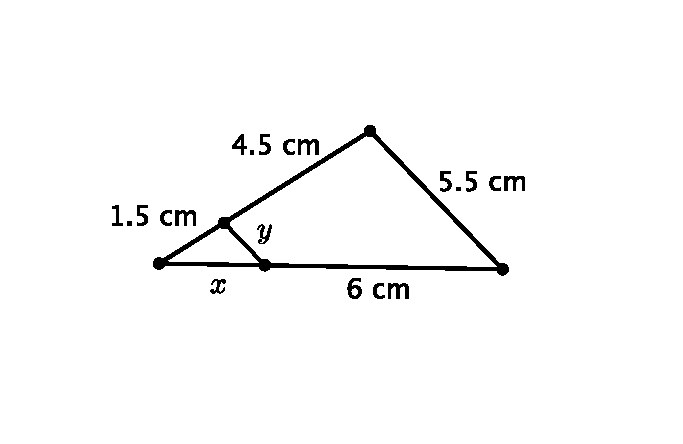
\includegraphics[width=0.35\textwidth]{img-09/trig-semblant3}
	\task   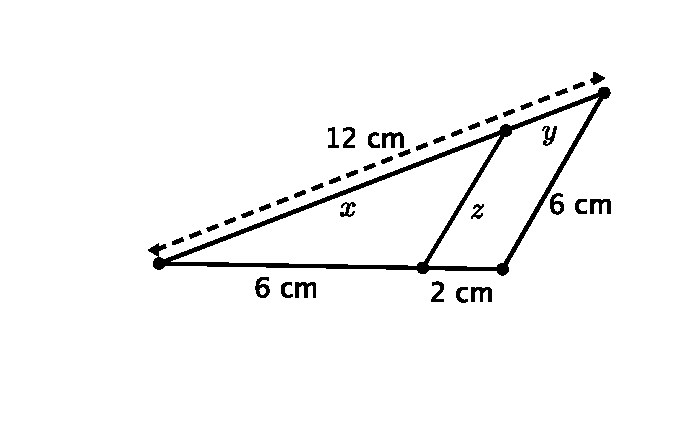
\includegraphics[width=0.4\textwidth]{img-09/trig-semblant4}
\end{tasks}

\answers[cols=1]{[$x=2$; $y=1.375$ cm,  $x=9$; $y=3$; $z=4.5$ cm]}

\end{mylist}
 


\section{Angles, longituds i àrees}

\begin{theorybox}
	Per qualsevol triangle, la suma dels seus angles és $\hat A + \hat B+ \hat C = 180^\circ$.
	
	\begin{minipage}{0.6\textwidth}
		Si un triangle té un angle de 90$^\circ$, \textbf{triangle rectangle}, podem aplicar el \textbf{teorema de Pitàgores}:
		\[a^2 = b^2 + c^2 \]
		on $a$ és la \textbf{hipotenusa} (el costat més llarg) i $b$ i $c$ els \textbf{catets}.
	\end{minipage}
\begin{minipage}{0.4\textwidth}
	\centering
	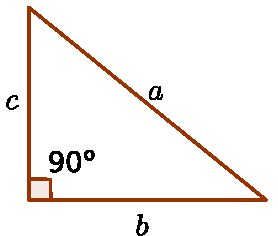
\includegraphics[width=0.8\textwidth]{img-09/pitagores}
\end{minipage}

Si sabem els catets, la hipotenusa s'obté de  $a=\sqrt{b^2+c^2}$.

Si ens falta un catet, aquest s'obté de $b=\sqrt{a^2-c^2}$  o $c=\sqrt{a^2-b^2}$ .
\end{theorybox}
 

\begin{mylist}
\exer  És possible trobar un triangle rectangle els catets del qual mesurin 5 i 12 cm i la seva hipotenusa 24 cm? Si la teva resposta és negativa, troba la mesura de la hipotenusa d'un triangle rectangle els catets del qual mesuren 5 i 12 cm. Utilitza calculadora per resoldre aquesta activitat si et resulta necessària. 

\answers{Sí. La hipotenusa ha de mesurar 13 cm}

\exer  Calcula la longitud de la hipotenusa dels següents triangles rectangles de catets:

\begin{tasks}(2)
	\task  6 cm i 8 cm   
	\task  4 m i 3 m
	\task  8 dm i 15 dm  
	\task  13,6 km i 21,4 km.
\end{tasks}
\answers[cols=2]{[10 cm, 5 m, 17 dm, 25.4 km]}

\exer  Calcula la longitud del catet que falta en els següents triangles rectangles d'hipotenusa i catet:

\begin{tasks}(2)
	\task  26 cm i 10 cm   
	\task  17 m i 8 m
	\task  37 dm i 35 dm  
	\task  14,7 km i 5,9 km
\end{tasks}
\answers[cols=2]{[24 cm,  15 m, 12 dm, 13.5 km]}

\exer[1] \hot  Calcula el costat $x$ del quadrat de la figura següent:
\begin{center}
 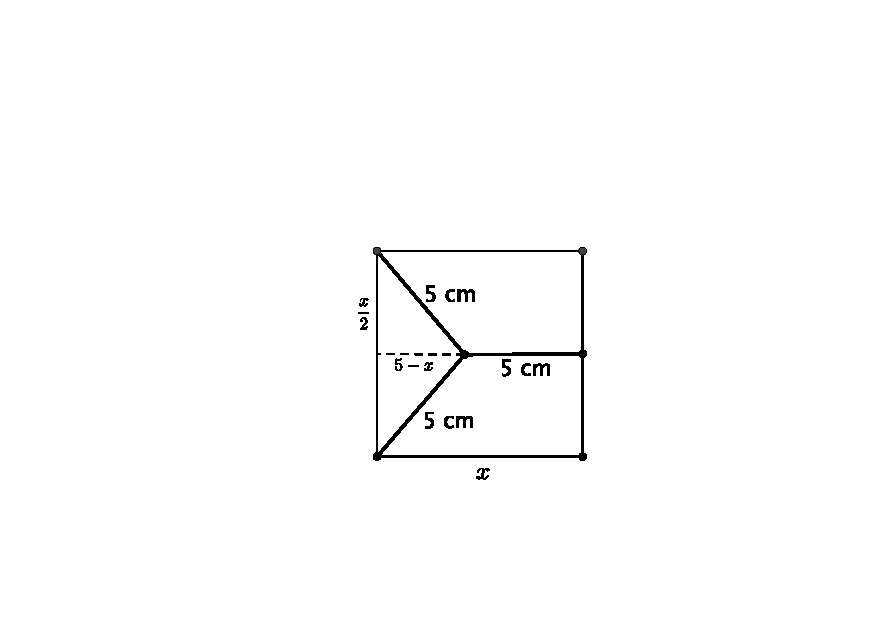
\includegraphics[width=0.2\textwidth]{img-09/fig6}
\end{center}
\answers{$x=8$ cm}

\end{mylist}
	
\begin{theorybox}[Fórmules àrees]	
	Trobareu un resum de les àrees de les figures planes a la pàgina \pageref{sec:resumarees}.
\end{theorybox}


\begin{mylist}

\exer  Calcula l'àrea d'un triangle equilàter de costat 9 m. 
\answers{$A=\frac{81}{4}\sqrt{3}=35.074$ cm$^2$.}

\exer  Calcula l'àrea d'un hexàgon regular de costat 2 cm. 
\answers{L'apotema és $a_p=1.732$. $A=6\sqrt{3}=10.39$ cm$^2$}

\exer  \hot Calcula el volum d'un tetraedre regular de costat 7 dm.
\answers{$V=\frac{1}{3}A_{base}H$. $A_{base}=21.218$, l'altura cau a 1/3 del costat la base $H=\frac{\sqrt{6}}{3}c=5.715$. $V=40.42$ dm$^3$}

\exer  Calcula la longitud de la diagonal d'un quadrat de costat 3 m.
\answers{$3\sqrt{2}=4.24$ m}

\exer  Calcula la longitud de la diagonal d'un rectangle de base 15 cm i altura 8 cm.
\answers{17 cm}

\exer  Una porteria de futbol mesura 7,32~m d'ample per 2,44~m d'alt. El punt de penal està a 11 metres. Calcula la distància que recorre la pilota en:

\begin{tasks}(2)
	\task  Un tir directe a la base del pal.

 
	\task  Un tir directe a l'esquadra.
\end{tasks}
\answers{[11.593 m, 11.84 m]}


\exer  Demostra que el diàmetre d'un quadrat de costat \textit{x} és $d=\sqrt{2} x$.
 

\exer  Demostra que l'altura d'un triangle equilàter de costat \textit{x} és $d=\frac{\sqrt{3} }{2} x$. 
 

\exer  Calcula els angles central i interior del triangle equilàter, quadrat, pentàgon regular, hexàgon regular i enneàgon regular.
\answers{120${}^\circ$ i 60${}^\circ$; 90${}^\circ$ i 90${}^\circ$; 72${}^\circ$ i 108${}^\circ$; 60${}^\circ$ i 120${}^\circ$; 40${}^\circ$ i 140${}^\circ$.}

\exer  Justifica que un hexàgon regular es pot descompondre en 6 triangles equilàters.
\answers{
	L'angle central mesura 60${}^\circ$. El triangle format per dos radis consecutius i el costat corresponent és
	isòsceles perquè tots els radis són iguals. L'angle suposadament desigual d'aquest triangle isòsceles
	mesura 60${}^\circ$ així que els altres dos angles també han de mesurar 60. Un triangle amb els tres angles iguals
	és equilàter.}

\exer  Demostra que l'altura d'un triangle equilater de costat a és $h=\sqrt{3} a/2$ i la seva àrea $A=\sqrt{3} a^2 /4$.
\answers{Mesura 73${}^\circ$}

\exer  Dos angles d'un trapezi isòsceles mesuren 35${}^\circ$  i 72${}^\circ$ , quant mesuren els angles que falten?

\answers{En un trapezi isòsceles els angles són iguals dos a dos i han de ser dos aguts i dos obtusos persumar en total 360. Aquest trapezi no pot ser isòsceles.}

\exer  Quant mesura la suma dels angles interiors d'un decàgon irregular? 
\answers{Els angles interiors sumen 1440${}^\circ$.}

\exer  Calcula l'àrea i el perímetre d'un trapezi isòsceles de bases 50 cm i 26 cm i altura 5 cm.
\answers{Àrea: 190 cm$^2$; perímetre: 133.28 cm.}

\exer  Calcula l'àrea i perímetre d'un trapezi rectangle de bases 100~cm i 64~cm, i d'altura 77~cm.
\answers{Àrea: 6314 cm$^2$; perímetre: 326 cm}
 
\exer  Calcula l'àrea i el perímetre d'un trapezi isòsceles de bases 100 cm i 60~cm i costats laterals 29~cm.
\answers{Àrea: 1 470 m$^2$; perímetre: 198 cm.}

\vspace{-1.5cm}
\exer[1] \begin{minipage}[t]{0.66\textwidth}
	 Utilitza el teorema de Pitàgores per determinar l'àrea i el perímetre de la zona ombrejada de la figura.
\end{minipage}
\begin{minipage}{0.3\textwidth}
	\centering
	\vspace{1.5cm}
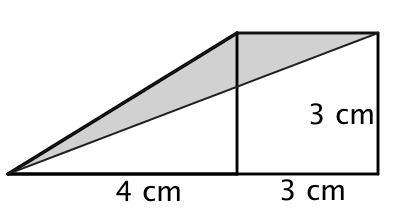
\includegraphics[width=0.8\textwidth]{img-09/fig7}
\end{minipage}
 \answers{$A=4.5$ cm$^2$, $P=15.62$ cm}
 
\exer  Tenint en compte que un hexàgon regular es pot dividir en sis triangles equilàters (l'altura de la qual és l'apotema de l'hexàgon regular), calcula l'àrea d'un hexàgon regular de 5 cm de costat.
\answers{El radi també és 5 cm i l'apotema $a_p=4.33$. L'àrea és: 64.95 cm$^2$}

\exer  Volem cobrir el pla amb polígons regulars de 100 cm${}^{2}$. Les úniques opcions possibles són el triangle equilàter, el quadrat i l'hexàgon. Calcula quina d'aquestes tres figures té menor perímetre. Quin animal aplica aquest resultat? [Utilitza la relació entre costat i altura d'un triangle equilàter obtinguda anteriorment]
\answers{L'hexàgon. Les abelles construeixen cel·les hexagonals.}

\exer  Tales va observar que en qualsevol triangle rectangle el circumcentre sempre estava en el punt mitjà de la hipotenusa. Comprova aquest resultat.
\answers{
	Veure la resposta següent.\par 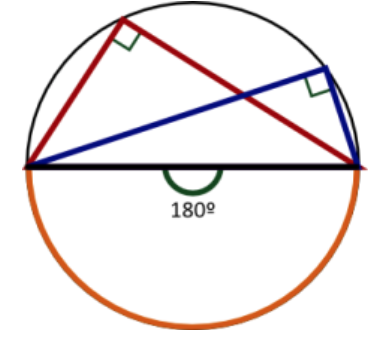
\includegraphics[width=0.34\textwidth]{img-sol/t9-32} \par La bisectriu de l'angle recte va del vèrtex al punt
	mitjà de la hipotenusa.}

\vspace{-1.5cm}
\exer \begin{minipage}[t]{0.7\textwidth}
	Un angle inscrit en la circumferència que abasta un diàmetre és un angle recte. Per què? Raona la resposta.
\end{minipage}
\begin{minipage}{0.3\textwidth}
	\centering
	\vspace{1.5cm}
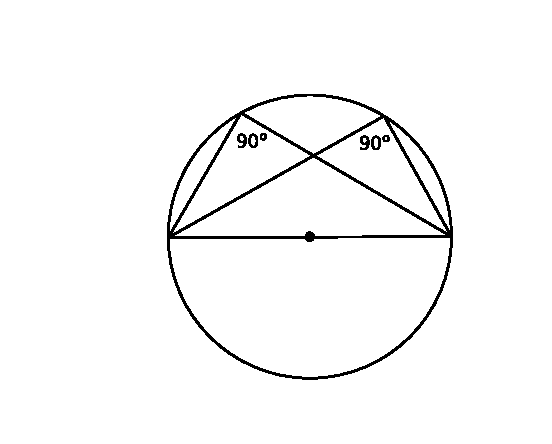
\includegraphics[width=0.7\textwidth]{img-09/fig8}
\end{minipage}

\answers{L'angle inscrit mesura la meitat que l'angle central. En aquest cas, la meitat de 180 és 90.} 

\exer  En quines posicions té un futbolista el mateix angle de tir que des del punt de penal?
\answers{
	Des de qualsevol punt de la circumferència circumscrita al triangle format per
	el punt de penal i les bases dels pals de la porteria. \par 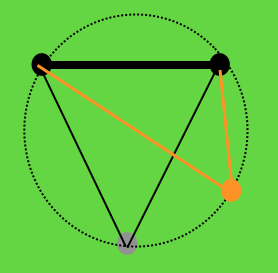
\includegraphics[width=0.35\textwidth]{img-sol/t9-33}}

\begin{comment}
\exer  \textit{Una altra demostració. Intenta comprendre-la. }Tracem un angle inscrit en la circumferència  CAB que tingui un costat que passi pel centre O de la circumferència. Tracem la seva central COB. El triangle OAC és isòsceles ja que dos dels seus costats són radis de la circumferència. Tracem per   O una recta paral·lela a AC. L'angle CAO és igual a l'angle DOB ja que tenen els seus costats paral·lels. L'angle ACO és igual a l'angle COD per alterns interns entre paral·leles, i és igual a l'angle CAO per ser el triangle isòsceles. Per tant el central mesura el doble que l'angle inscrit. 


\exer   Les circumferències de grandària real de la il·lustració del marge tenen com a radi, la menor 1 cm, la següent, una mica més fosca 2 cm, la clara següent 3 cm, i així, augmenta un centímetre. Calcula les longituds de les 10 primeres circumferències. 7

\end{comment}
 


\exer  La Terra és aproximadament una esfera de radi 6.379 km. Quant mesura l'Equador?
\answers{$L=2\pi \cdot 6379 = 40080.44$ km}

\exer  Antigament es definia un metre com: ``\textit{la deu milionèsima part del quadrant del meridià terrestre que passa per París}''. Segons aquesta definició, quant mesura (en metres) el diàmetre terrestre? 
\answers{6366 km}

\exer   Un far gira descrivint un arc de 170${}^\circ$ . A una distància de \textit{5 km}, quina és la longitud de l'arc de circumferència en el qual es veu la llum?
\answers{Aproximadament 14.8 km}

\exer  Determina l'àrea  del triangle equilàter de 10 cm de radi.
\answers{$A=43.3$ cm$^2$}

\exer  Calcula l'àrea tancada per una circumferència de radi 9 cm.
\answers{$A=254.47$ cm$^2$}

\exer  Calcula l'àrea de la corona circular de radis 12 i 5 cm.
\answers{$A=119\pi=376.85$ cm$^2$}

\exer  Calcula l'àrea del sector circular i del segment circular de radi 6 cm i que forma un angle de 60${}^\circ$ . 
\answers{Sector: 18.85 cm$^2$ i el segment 3.26 cm$^2$}

\exer  Calcula l'àrea del sector de corona circular de radis 25 cm i 18 cm i que forma un angle de 60${}^\circ$ . 
\answers{$301\frac{\pi}{6}=157.60$ cm$^2$}

\exer[1]  Calcula l'àrea tancada entre aquests cercles de 5~cm de radi.
\begin{center}
	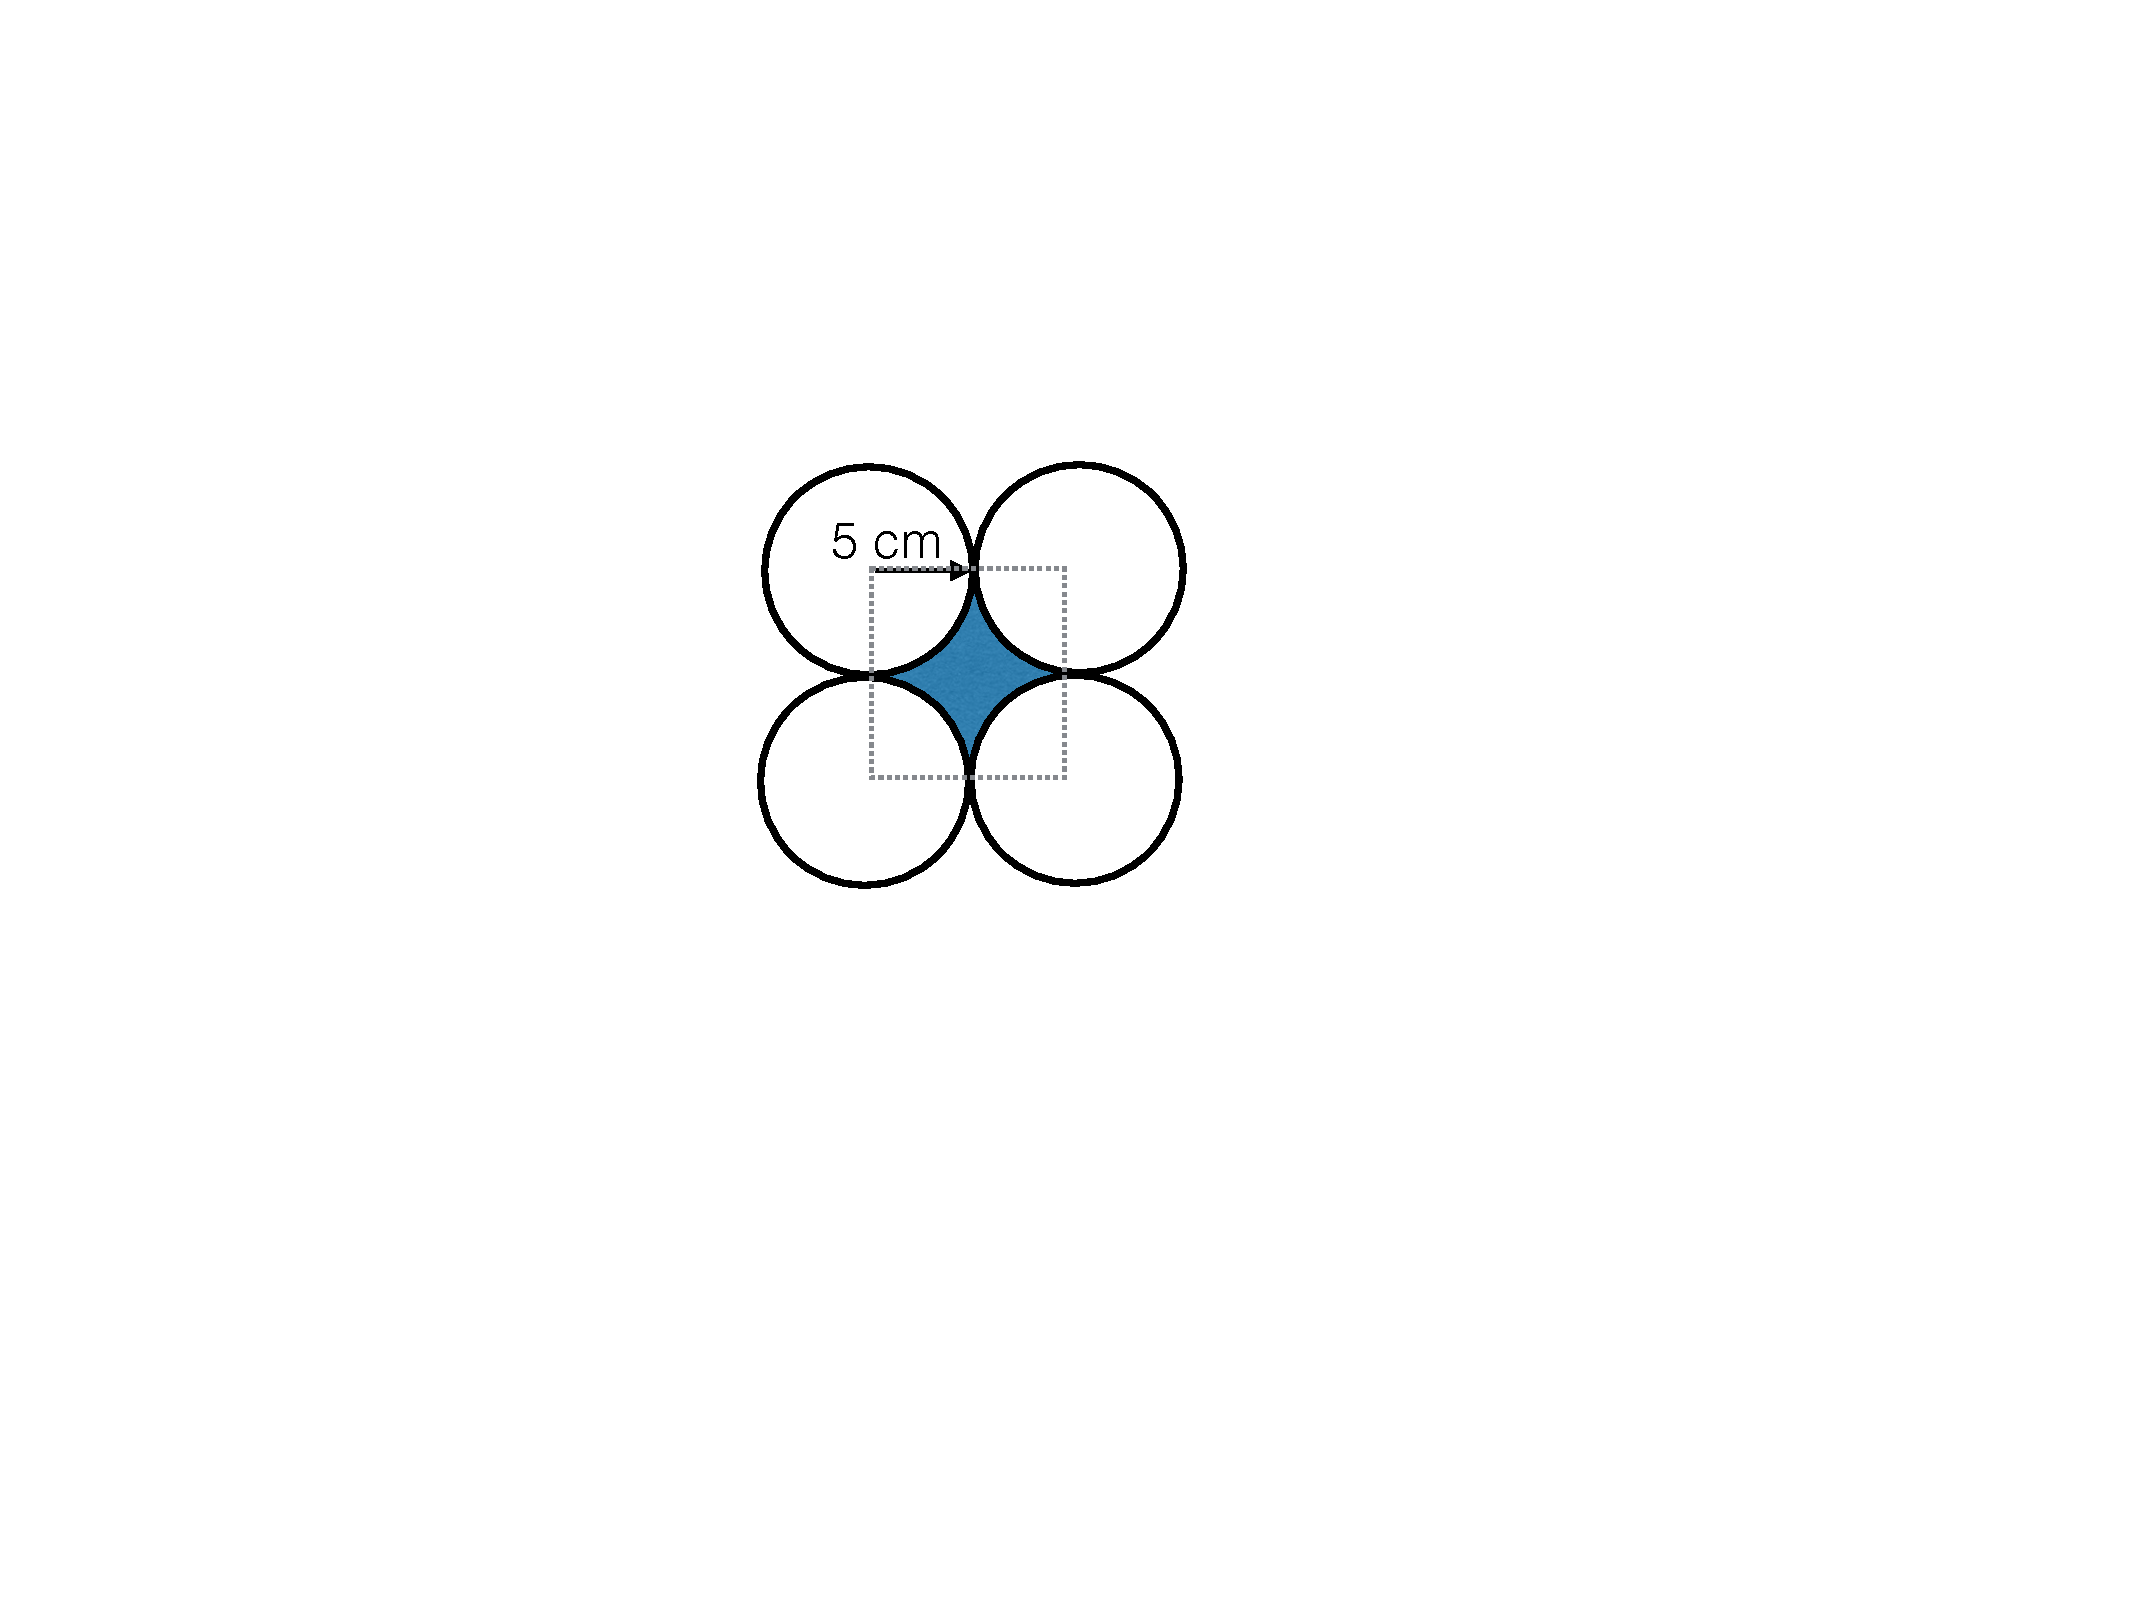
\includegraphics[width=0.2\textwidth]{img-09/fig9}
\end{center}
 \answers{$A=10^2-\pi 5^2=21.46$ cm$^2$}

\vspace*{-1.5cm}
\exer \begin{minipage}[t]{0.7\textwidth}
	Una figura típica de l'arquitectura gòtica es dibuixa a partir d'un triangle equilàter traçant arcs de circumferència amb centre en cadascun dels seus vèrtexs i que passen pels dos vèrtexs restants. Calcula l'àrea d'una d'aquestes figures si es construeix a partir d'un triangle equilàter de 2 metres de costat. Calcula l'àrea tancada entre aquests cercles de 5~cm de radi.
\end{minipage}
\begin{minipage}{0.3\textwidth}
	\centering
	\vspace{2cm}
	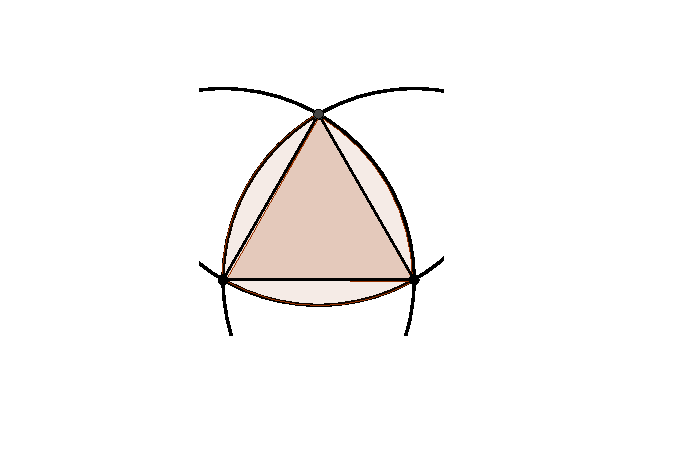
\includegraphics[width=0.6\textwidth]{img-09/fig10}
\end{minipage}

\answers{En general $\frac{R^2}{2}(\pi - \sqrt{3})=1.41$ m$^2$}
  
 \vspace*{-1.5cm}
 \exer \begin{minipage}[t]{0.7\textwidth}
 	Calcula l'àrea i el perímetre de la figura formada per un triangle equilàter de 8~cm de costat sobre el qual es construeix un sector circular. 
 \end{minipage}
 \begin{minipage}{0.3\textwidth}
 	\centering
 	\vspace{1.5cm}
 	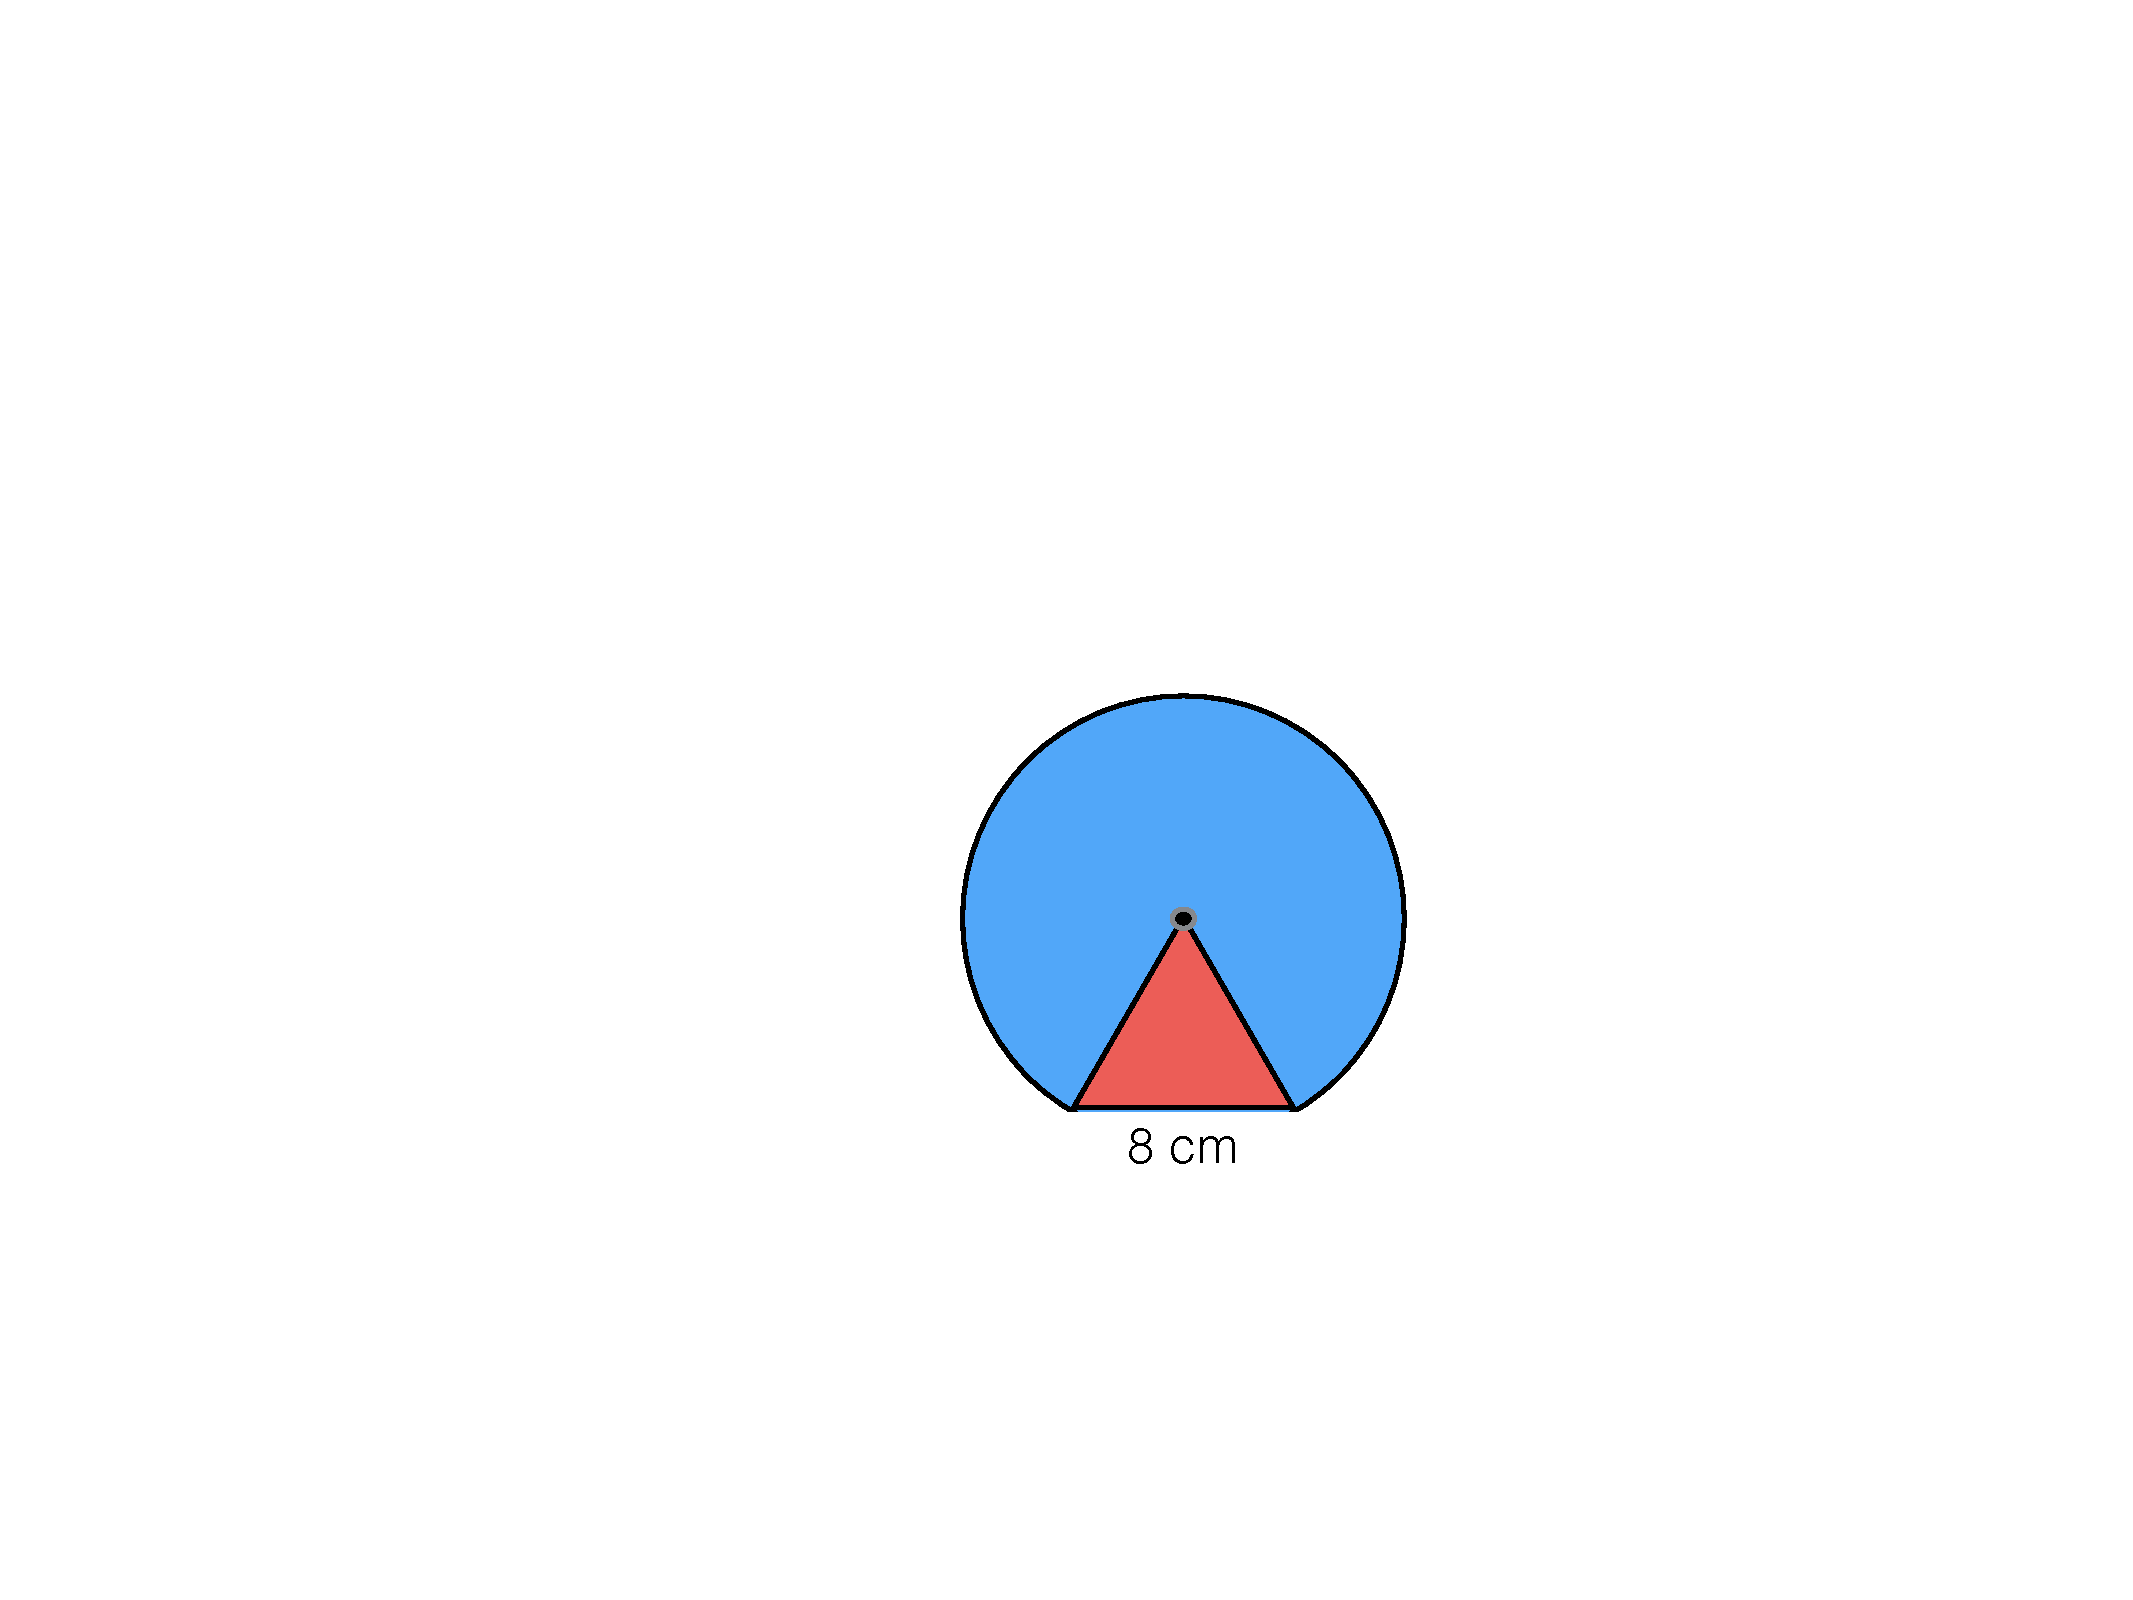
\includegraphics[width=0.5\textwidth]{img-09/fig11}
 \end{minipage}
 
 \answers{$64\cdot \left(\frac{5\pi}{6} + \frac{\sqrt{3}}{4} \right)=195.26$ cm$^2$}
 
\vspace*{-1.5cm}
\exer \begin{minipage}[t]{0.7\textwidth}
	 Hi ha 5 circumferències inscrites en una circumferència de 12~cm de radi tal com indica la figura. Quant val l'àrea ombrejada?
\end{minipage}
\begin{minipage}{0.3\textwidth}
	\centering
	\vspace{1.5cm}
	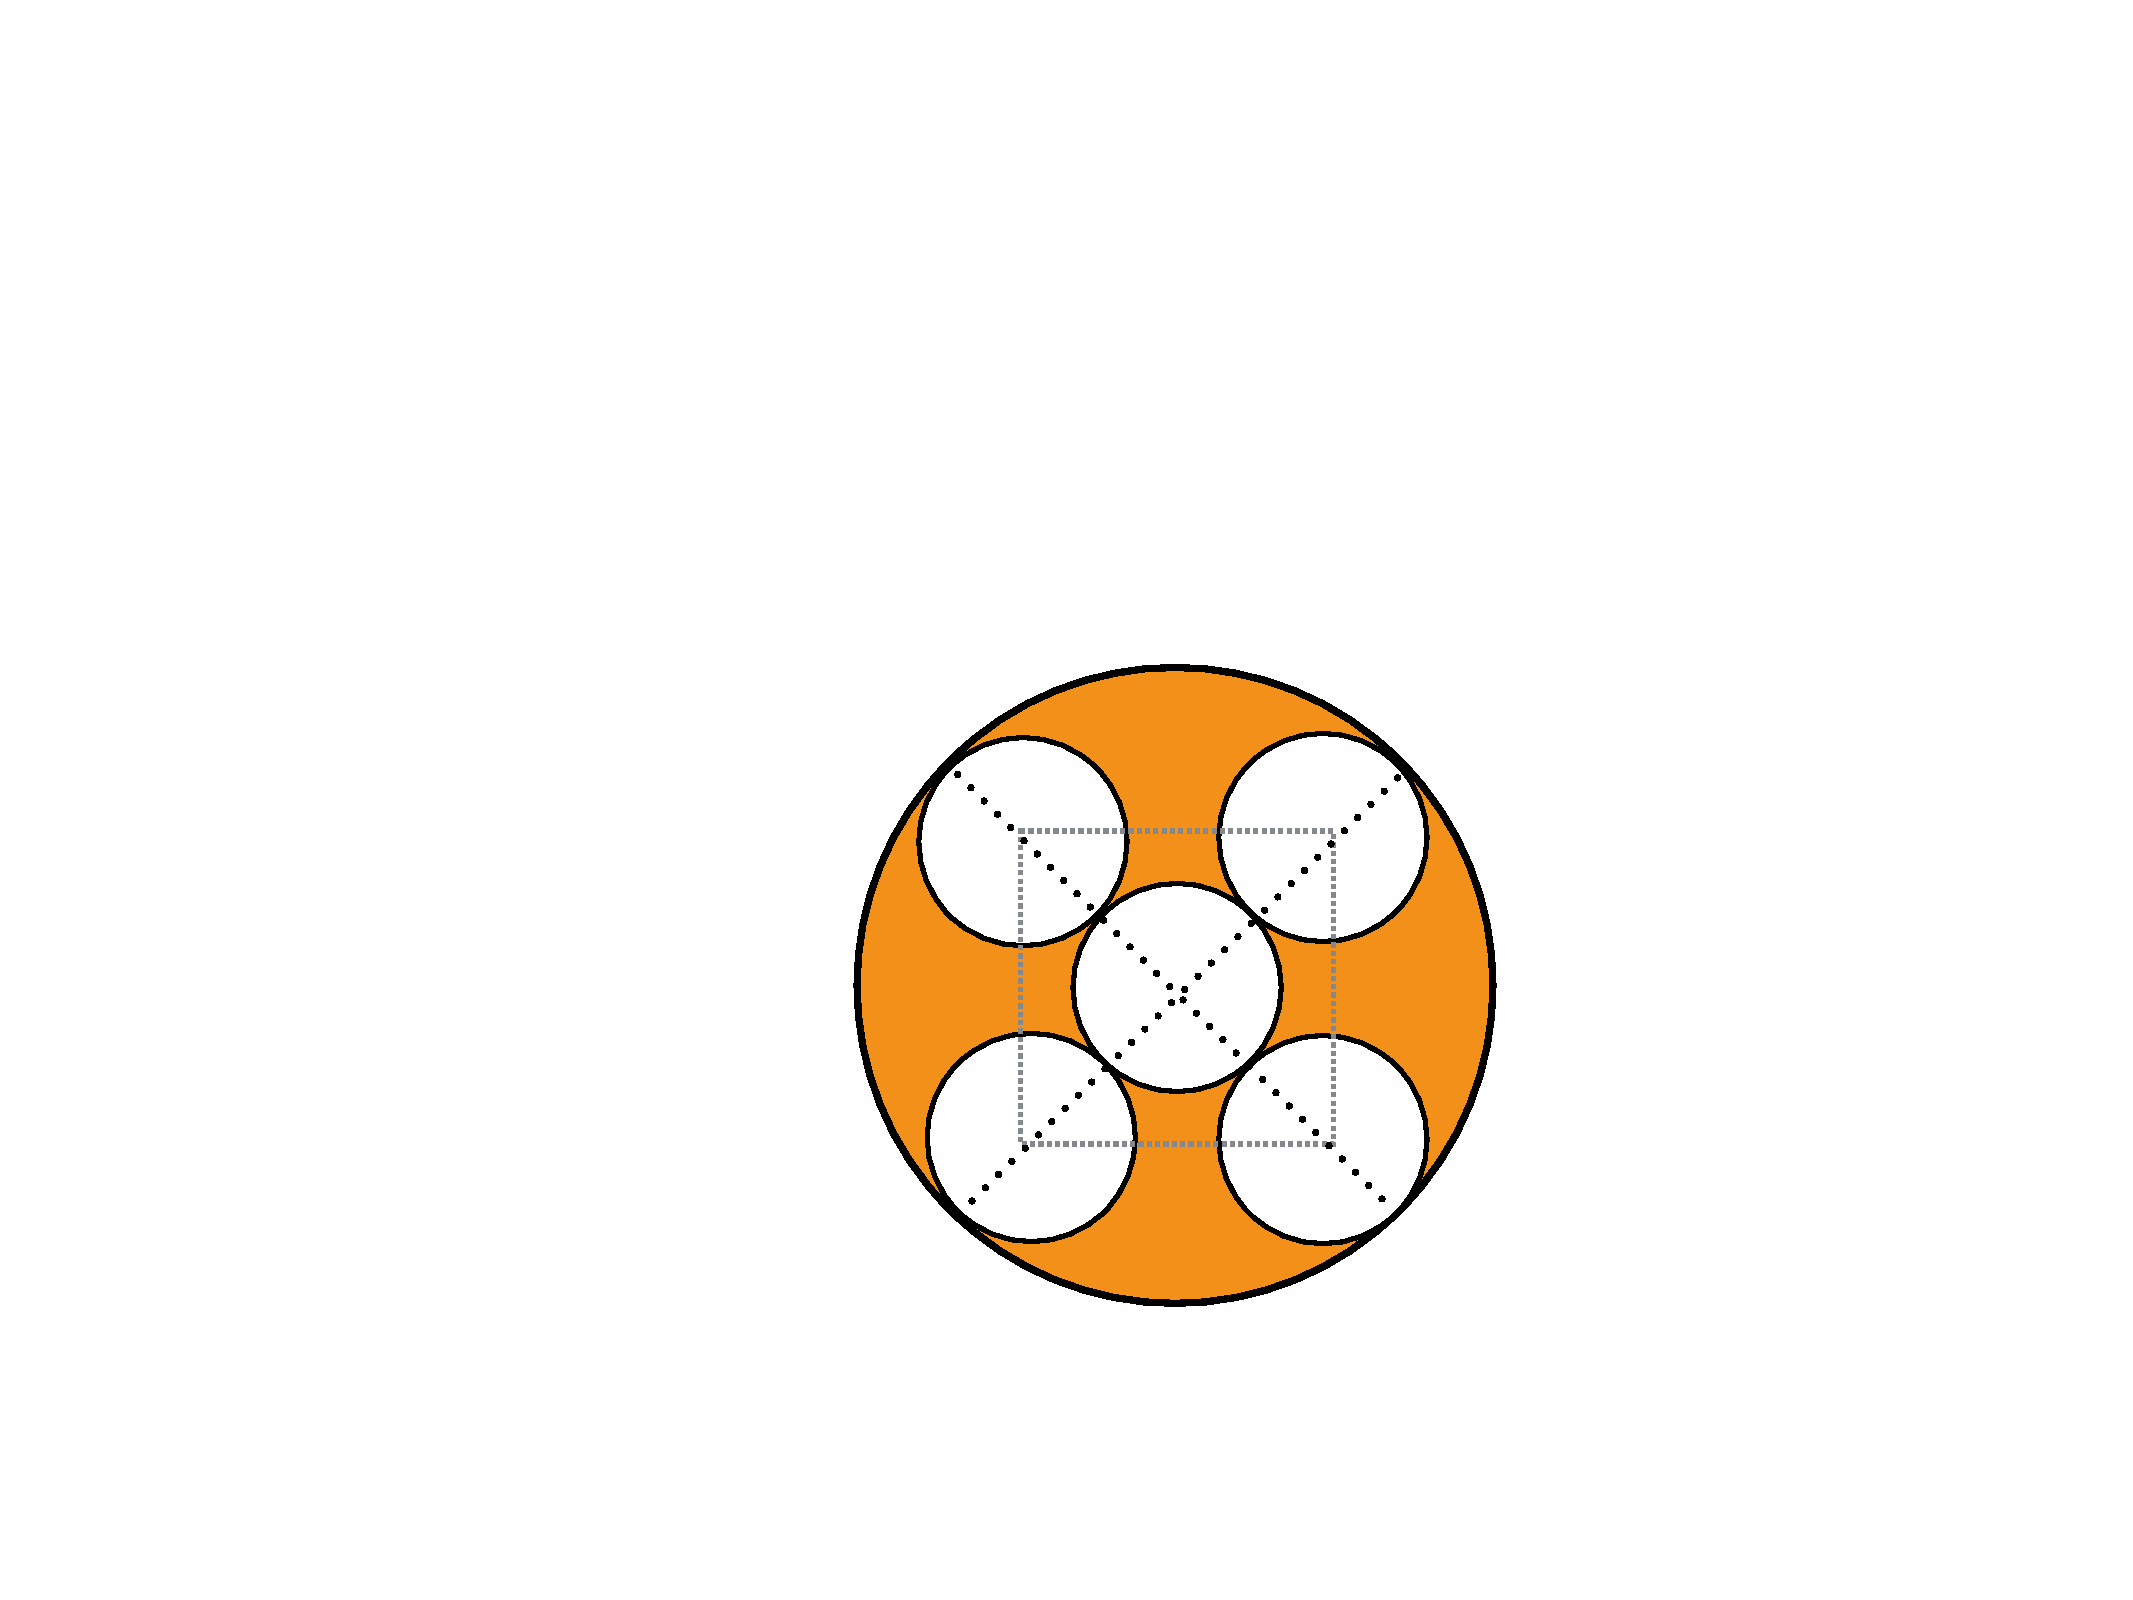
\includegraphics[width=0.5\textwidth]{img-09/fig12}
\end{minipage}
 
 \answers{$A=\pi \cdot 12^2 - 5 \pi \cdot 4^2=64 \cdot \pi=201.06$ cm$^2$}
 
\vspace*{-1.5cm}
\exer \begin{minipage}[t]{0.7\textwidth}
	Un formatge cilíndric té una base circular de 14~cm de diàmetre i una etiqueta circular de 8~cm de diàmetre. Es talla un tascó de 70${}^\circ$ . Quina àrea té el tros d'etiqueta tallada? 
	
\end{minipage}
\begin{minipage}{0.3\textwidth}
	\centering
	\vspace{1.5cm}
	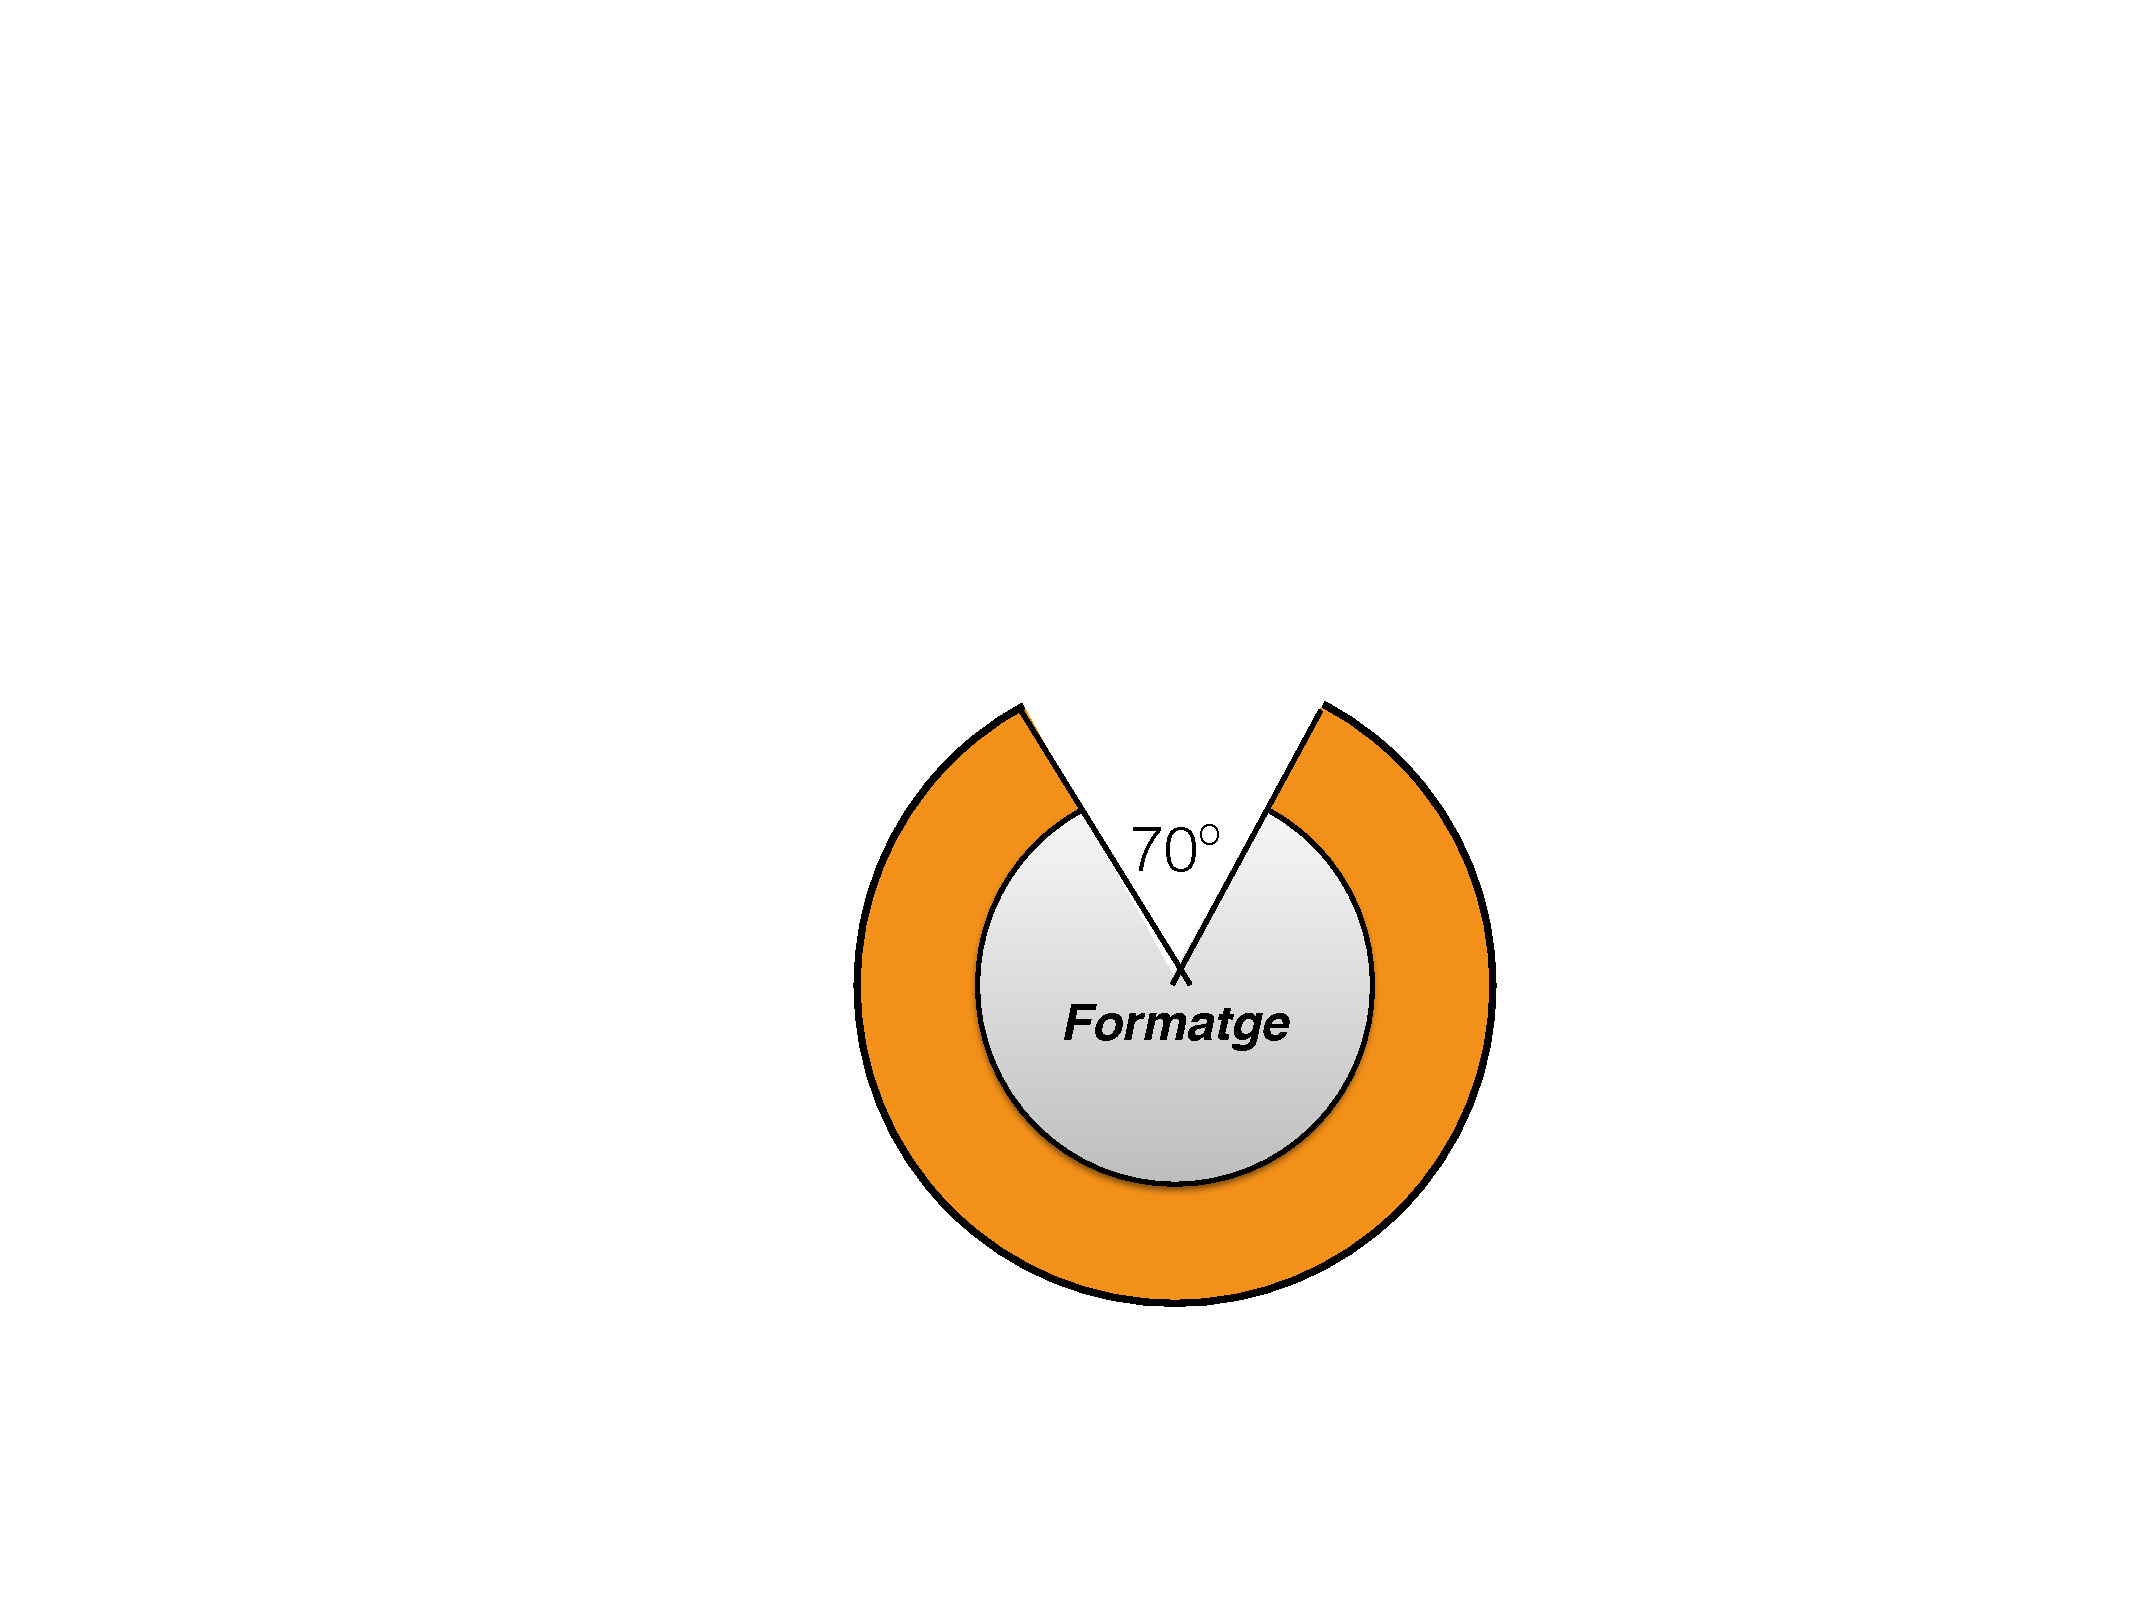
\includegraphics[width=0.5\textwidth]{img-09/formatge}
\end{minipage}
 
 \answers{$A=\frac{24\pi}{9}=9.77$ cm$^2$}
  
\pagebreak
\mbox{}
 
\vspace*{-1.5cm}
\exer[1] \begin{minipage}[t]{0.62\textwidth}
	A partir d'un triangle rectangle isòscels de 3~cm de catet construïm un sector circular. Calcula l'àrea de la figura.
\end{minipage}
\begin{minipage}{0.3\textwidth}
	\centering
	\vspace{1.5cm}
	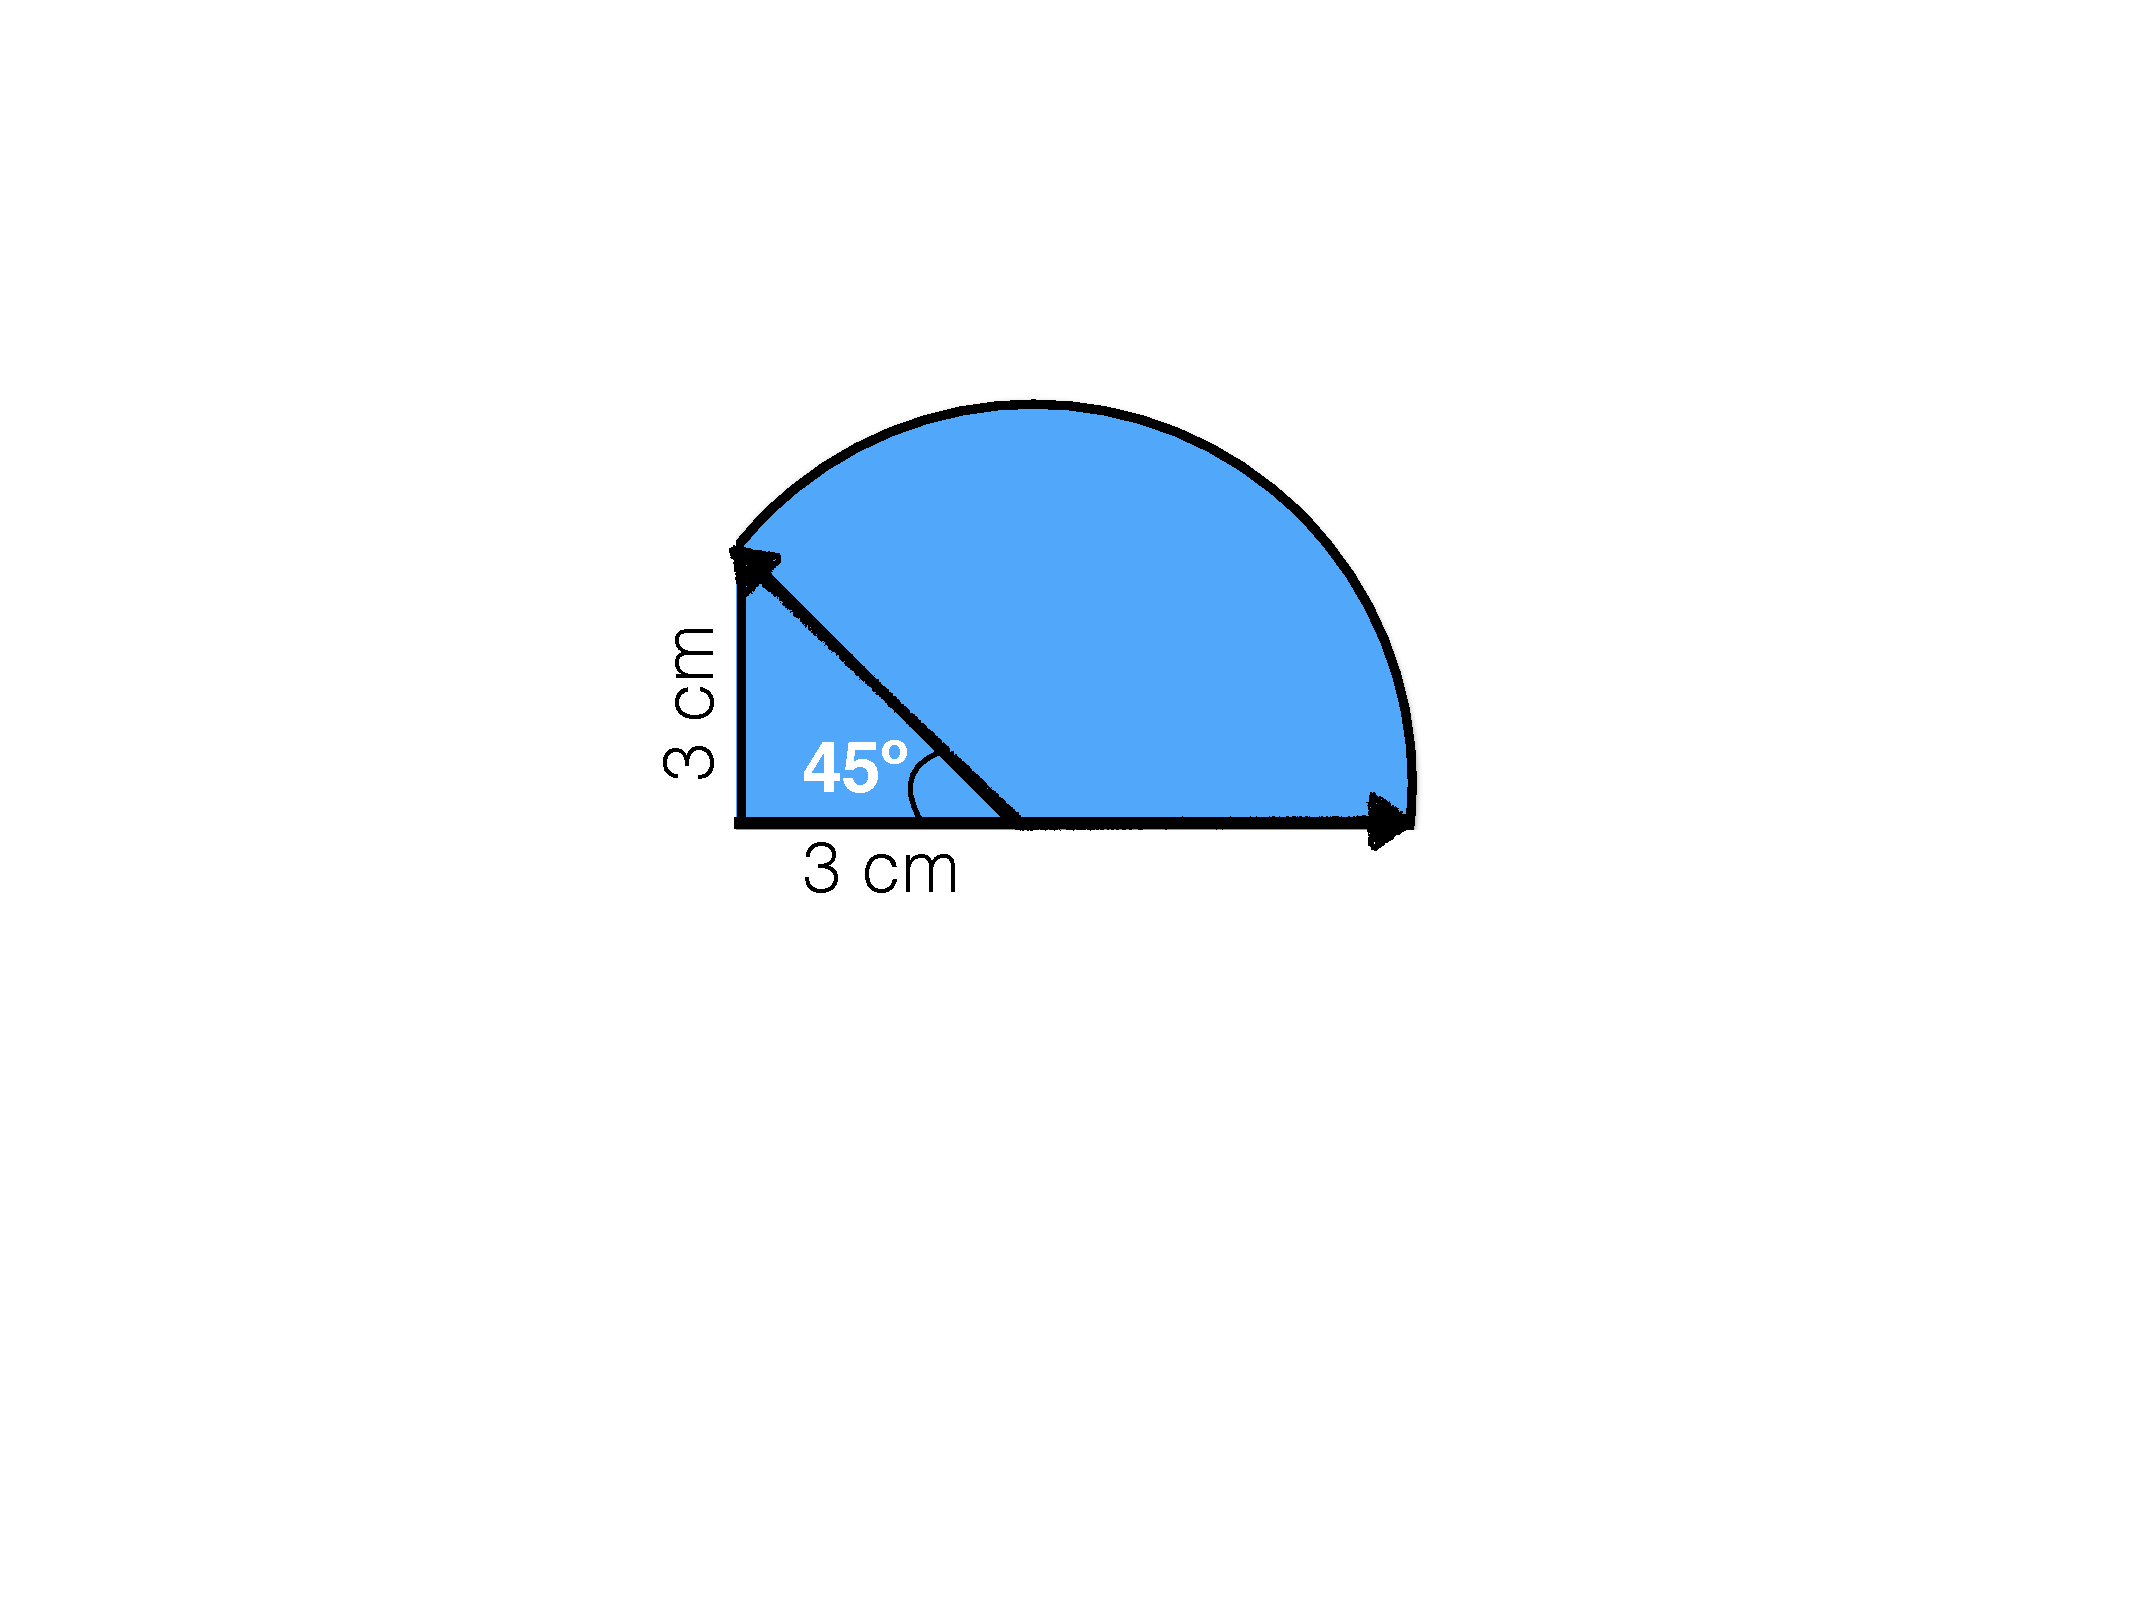
\includegraphics[width=0.7\textwidth]{img-09/fig14}
\end{minipage}
 \answers{$A=\frac{9}{2}+ \frac{135}{360} \cdot \pi \cdot 18 = 25.71$ cm$^2$}
 
 
\vspace{-1.5cm}
\exer \hot \begin{minipage}[t]{0.62\textwidth}
	En dues rectes que formen 60${}^\circ$,  s'inscriuen dues circumferències tangents entre si.  La primera té el centre a 2~centímetres del vèrtex i el radi de 1~centímetre. La segona  té de radi 3~centímetres. Quant val l'àrea ombrejada? 
	
\end{minipage}
\begin{minipage}{0.3\textwidth}
	\centering
	\vspace{1.5cm}
	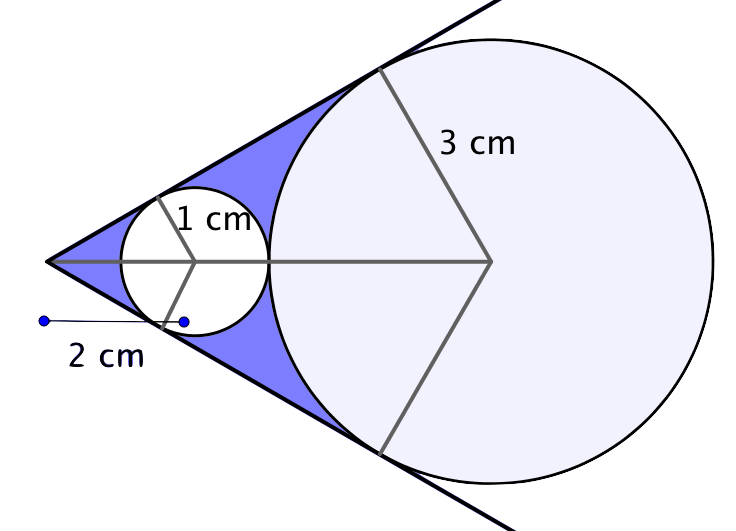
\includegraphics[width=0.99\textwidth]{img-09/fig16}
\end{minipage}
 
 \answers{$A=9\sqrt{3}-4\pi=3.02$ cm$^2$}
 
 \vspace{-1.5cm}
 \exer[1] \begin{minipage}[t]{0.62\textwidth}
	  Tracem tres arcs circulars des de tres vèrtexs d'un hexàgon de 5~cm de costat. 
	  Calcula l'àrea i el perímetre exterior de la figura.
 \end{minipage}
 \begin{minipage}{0.3\textwidth}
 	\centering
 	\vspace{1.5cm}
 	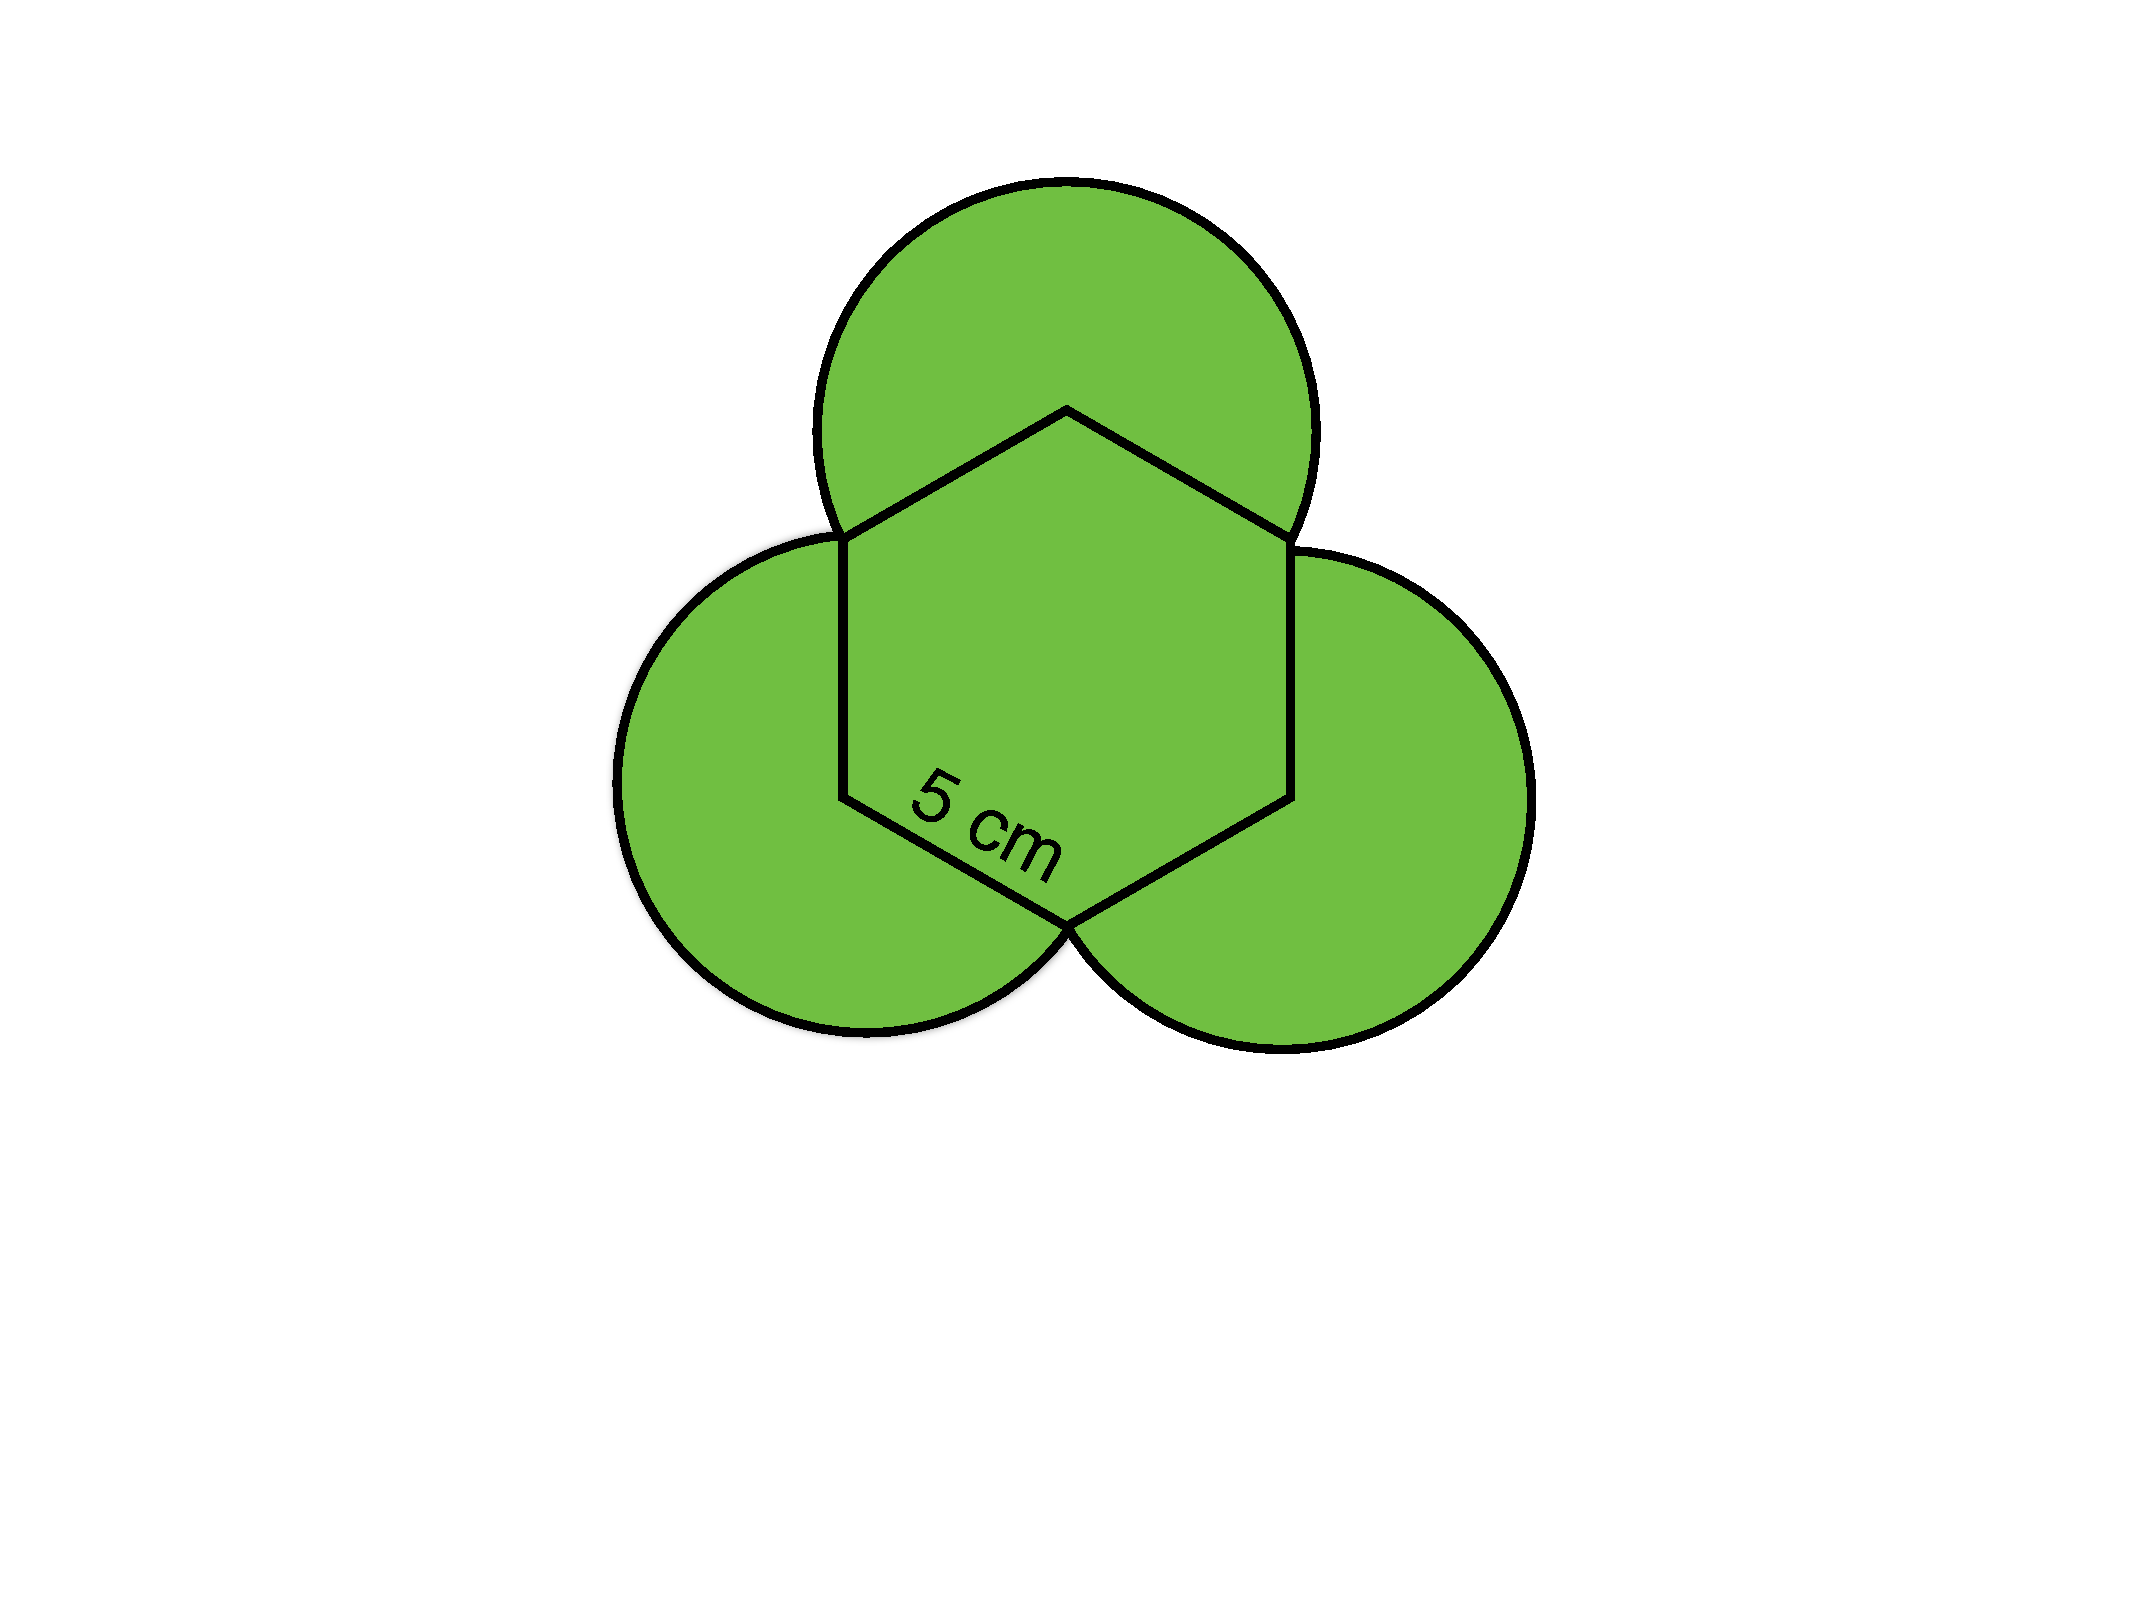
\includegraphics[width=0.6\textwidth]{img-09/fig15}
 \end{minipage}
\answers{$P=62.83$ cm i $A=222.03$ cm$^2$}
  
 
\end{mylist}
 
\section{Llocs geomètrics}

\begin{theorybox}
	Un \textbf{lloc geomètric} està format per un conjunt de punts del pla que compleixen una determinada condició.
	
	\begin{itemize}	
		\item \textbf{Circumferència}: Està format per tots els punts del pla que equidisten d'un punt anomenat centre. Aquesta distància li deim radi.
		
		\item \textbf{Mediatriu}: Conjunt de punts que equidisten dels extrems d'un segment $\overline{AB}$. És una recta que passa pel punt mitjà $M=\frac{A+B}{2}$ del segment i és perpendicular a ell.
		
		\item \textbf{Bisectriu}: Conjunt de punts que equidisten de dues rectes. És una recta que divideix un angle en dues parts iguals.
\end{itemize} 
\end{theorybox}

\begin{theorybox}
		
		\begin{multicols}{3}
			\footnotesize
			\centering
			
			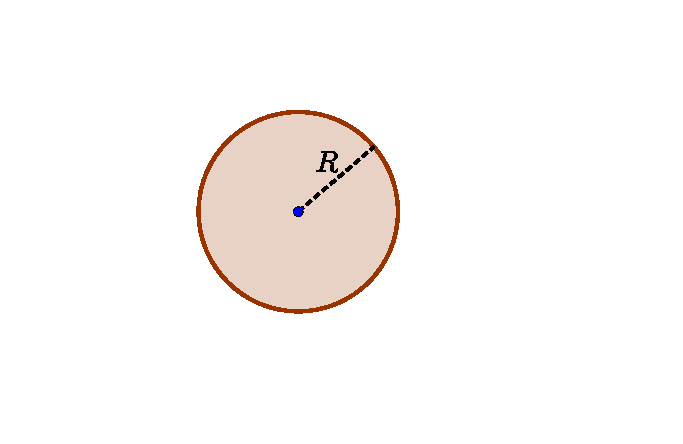
\includegraphics[height=2.5cm]{img-09/cercle}
			
			Circumferència
			
			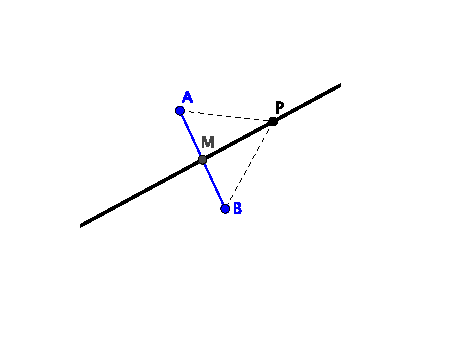
\includegraphics[height=2.5cm]{img-09/mediatriu}
			
			Mediatriu
			
			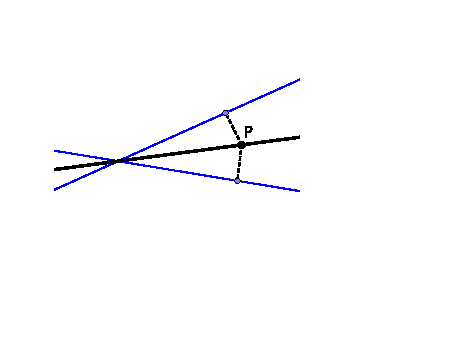
\includegraphics[height=2.5cm]{img-09/bisectriu}
			
			Bisectriu
		\end{multicols}

\end{theorybox}

\pagebreak

\begin{theorybox}
	Considerau un triangle de vèrtexs $ABC$:
	\begin{itemize}	
		\item \textbf{Mediana al costat $AB$}: és la recta que passa pel punt mitjà del segment $\overline{AB}$ i pel vèrtex oposat $C$.
		
		\item \textbf{Altura al costat $AB$}: És la recta que passa pel vèrtex oposat $C$ i és perpendicular al segment $\overline{AB}$.
	\end{itemize}
	
	Si en un triangle hi dibuixam les tres \textbf{mediatrius} als seus treus costats veim que es tallen en un punt anomenat \textbf{circumcentre} (O). El circumcentre és el centre de la circumferència circumscrita en el triangle.
	
	Si en un triangle hi dibuixam les tres \textbf{bisectrius} interiors als seus treus angles veim que es tallen en un punt anomenat \textbf{incentre} (I). L'incentre és el centre de la circumferència inscrita en el triangle.
	
	Si en un triangle hi dibuixam les tres \textbf{medianes} als seus treus costats veim que es tallen en un punt anomenat \textbf{baricentre} (G). El baricentre és el centre de gravetat del triangle.
	
	Si en un triangle hi dibuixam les tres \textbf{altures} als seus treus costats veim que es tallen en un punt anomenat \textbf{ortocentre} (H). 
	
	\begin{multicols}{2}
		\footnotesize
		\centering
		
		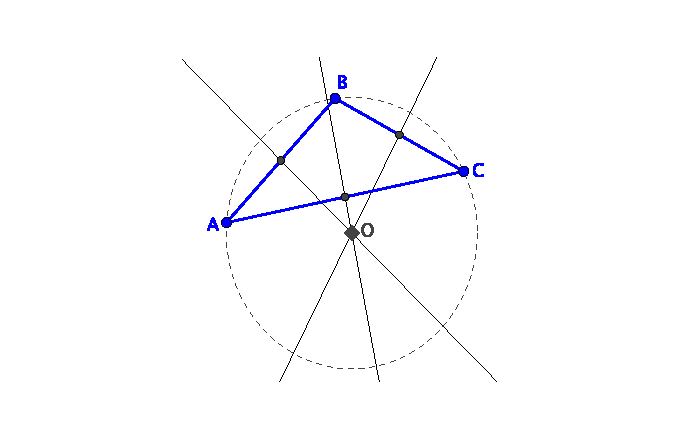
\includegraphics[height=3.5cm]{img-09/circumcentre}
		
		Mediatrius -- Circumcentre
		
		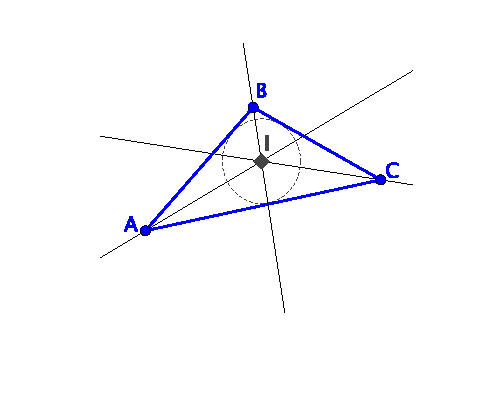
\includegraphics[height=3.5cm]{img-09/incentre}
		
		Bisectrius -- Incentre
		
		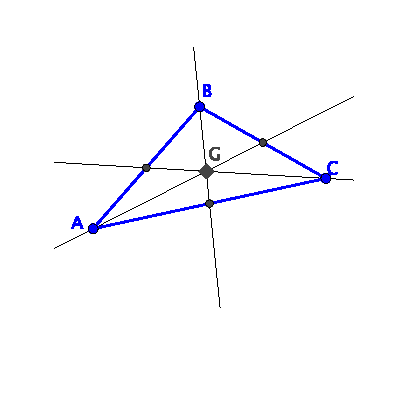
\includegraphics[height=3.5cm]{img-09/baricentre}
		
		Medianes -- Baricentre
		
		
		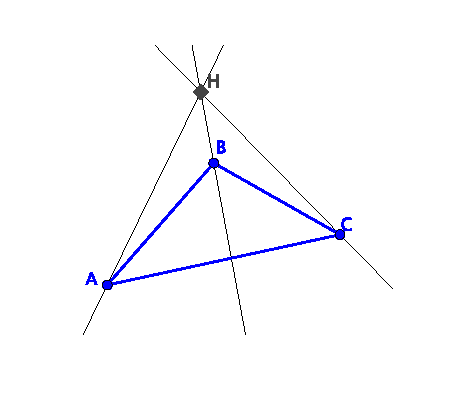
\includegraphics[height=3.5cm]{img-09/ortocentre}
		
		Altures -- Ortocentre
		
	\end{multicols}
	
\end{theorybox}
 
\begin{mylist}
 
	\exer  Dibuixa un triangle isòsceles amb l'angle desigual de 40${}^\circ$ . Traça les rectes notables per al costat desigual i per a un dels costats iguals. Què passa?
	
	\answers{
		L'altura corresponent al costat desigual és també mitjana, mediatriu i bisectriu. Les altres rectes
		notables no coincideixen.}
	
	\exer  Volem situar un fanal en una plaça triangular. On el posaríem?
	
	\answers{	Si la posem al circumcentre, els tres vèrtex rebran la mateixa llum, però pot ser molt poca si es
		tracta d'un triangle obtusangle (el circumcentre quedarà fora de la plaça). Si la posem en l'incentre,
		tindrem un cercle complet de bona llum dins de la plaça, però no necessàriament en els vèrtexs.}
	
	\exer  Una formiga camina per una mediana d'un triangle partint del vèrtex. Quan arriba al baricentre ha recorregut 8 centímetres. Quina distància li falta per arribar al punt mitjà del costat oposat al vèrtex d'on va partir?
	
	\answers{Ha recorregut 4 cm}
	
	\exer  Tenim un camp triangular sense tancar i volem lligar una cabra de manera que no surti del camp però que accedeixi al màxim de pastura possible. On posaríem el pal?
	
	\answers{En l'incentre}
	
	\exer  Na Iaissa i al seu germà Aitor els encanta el pastís. La seva mare els ha fet un triangular. Iassa l'ha de tallar però Aitor triarà primer el seu tros. Com hauria de tallar Iaissa el pastís?
	
	\answers{Ha de seguir una de les medianes}
	
	\exer  Comprova que el circumcentre d'un triangle rectangle està sempre en el punt mitjà de la hipotenusa. On està l'ortocentre?
	
	\answers[cols=1]{[
		L'angle central corresponent a un angle inscrit d'90$^\circ$ mesura 180$^\circ$. Per tant la hipotenusa del triangle ha de ser un diàmetre de la circumferència., L'ortocentre es troba en el vèrtex de l'angle recta.]}
	
	\exer  El baricentre és el centre de gravetat. Construeix un triangle de cartolina i dibuixa el seu baricentre. Si poses el triangle horitzontalment en l'aire només subjectat per la punta d'un llapis en el baricentre comprovaràs que se subjecta. 
	
	\answers{Solució manipulativa}
	
	\exer  Calcula el costat d'un triangle equilàter inscrit en una circumferència de 10~cm de radi. [\textit{Ajuda}: Aplica que en aquest cas el circumcentre coincideix amb el baricentre i que aquest últim està al doble de distància del vèrtex que del costat oposat.] 
	
	\answers{$20\sqrt{3}$ cm}
	
	\exer \ggb El \textit{baricentre} divideix a la mediana en dues parts, essent una part dos terços de l'altra. Comprova-ho.
	
	\answers{Solució manipulativa utilitzant Geogebra}
	
	\exer \simbolsearch La recta de \textit{Euler} passa \textit{pel circumcentre}, el \textit{baricentre} i l'ortocentre, però l'incentre no sempre pertany a la recta de \textit{Euler}. Com ha de ser el triangle perquè hi pertanyi? 
		
	\answers{Solució manipulativa utilitzant Geogebra: El triangle ha d'ésser isòscels}
 
	\exer  Un agricultor troba en el seu camp una bomba de la Guerra Civil. Les autoritats estableixen una distància de seguretat de 50 metres. Com s'ha d'acordonar la zona?
	
	\answers{Una circumferència en centre la bomba i radi 50 m.}
	
	\exer  Un joc de dos participants consisteix que se situen a una distància de dos metres entre ells i es posen diverses banderes a la mateixa distància de tots dos. La primera a 5 metres, la segona a 10 metres, la tercera a 15 i així successivament. Sobre quina línia imaginària estarien situades les banderes?
	
	
	\answers{A la mediatriu del segment, els extrems són els dos participants.}
	
	
	\exer  Quan en una acampada ens seiem al voltant del foc ho fem formant un cercle. Per què?
	
	 
	\answers{Ens trobam a igual distància del centre i per tant rebem la mateixa quantitat de calor.}
	
	\exer  Utilitza regla i compàs per dibuixar la bisectriu d'un angle i la mediatriu d'un segment.
	
	\answers{Resposta gràfica}
	
	\exer  Dibuixa en el teu quadern un triangle de costats 7, 6 i 4 cm. Traça en ell les circumferències inscrites i circumscrites.
	
	\answers{Resposta gràfica}
	
	\exer  Dibuixa en el teu quadern un triangle de costat 8 cm i angles adjacents al mateix de 40${}^\circ$  i 30${}^\circ$ . Troba el seu ortocentre i el seu baricentre.
	
	\answers{Resposta gràfica i manipulativa}
	
	\exer  Dibuixa en el teu quadern un triangle amb un angle de 40${}^\circ$  comprès entre dos costats de 6 i 4 cm. Obté el seu circumcentre i el seu incentre.
	
	\answers{Resposta gràfica i manipulativa}
	
	\exer  Com són les rectes i els punts notables en un triangle equilàter?
	
	\answers{
		Les medianes són també mediatrius, bisectrius i altures. Els quatre punts notables coincideixen.}
	
\end{mylist}

 
\pagebreak

\begin{activitats}


\subsection{Semblança}
\begin{mylist}
\exer  Indica si són semblants els següents parells de triangles:

\begin{tasks}
	\task  Un angle de 70${}^\circ$  i un altre de 20${}^\circ$ . Un angle de 90${}^\circ$  i un altre de 20${}^\circ$ . 
	\task  Triangle isòsceles amb angle desigual de 80${}^\circ$ . Triangle isòsceles amb un angle igual de 50${}^\circ$ .
	\task  \textit{A =} 40${}^\circ$ , \textit{b} = 8 cm, \textit{c} = 10 cm. \textit{A'}= 40${}^\circ$ , \textit{b}' = 4 cm, \textit{c}' = 5 cm
	\task  \textit{a =} 3 cm, \textit{b} = 4 cm, \textit{c} = 6 cm. \textit{a'} = 9 cm, \textit{b'} = 12 cm, \textit{c'} = 19 cm 
\end{tasks}

\answers[cols=2]{[Sí, Sí, Sí, No]}

\exer  Calcula el valor desconegut perquè els triangles siguin semblants:

\begin{tasks}
	\task  \textit{a =} 15 cm, \textit{b} = 9 cm, \textit{c} = 12 cm. \textit{a}' = 10 cm, \textit{b'} = 4 cm, \textbf{\textit{c'=}?}
	\task  \textit{A =} 50${}^\circ$ , \textit{b} = 6 cm, c = 4 cm. \textit{A'} = 50${}^\circ$ , \textit{b'} = 18 cm, \textbf{\textit{a'=}?}
\end{tasks}
\answers[cols=1]{[No es pot trobar $c'$ perquè no són semblants $\frac{15}{10}\neq \frac{9}{4}$, $a'=12$ cm]}


\exer  Les longituds dels costats d'un triangle són 12 cm, 14 cm i 14 cm. Un triangle semblant a ell té un perímetre de 90 cm. Quant mesuren els seus costats?
\answers{27, 31.5 i 31.5 cm}

\exer  Dibuixa en el teu quadern un pentàgon regular. Traça les seves diagonals. El triangle format d'una banda del pentàgon i les dues diagonals del vèrtex oposat es denomina triangle auri, ja que en dividir el costat major entre el menor s'obté el nombre d'or, quant mesuren els seus angles? Cerca en la figura que has traçat altres triangles auris. Quina és la relació de proporcionalitat? 
\answers{Els angles són 36, 72 i 72 graus.}

\exer  L'ombra d'un edifici mesura 15 m, i la del primer pis 2 m. Sabem que l'altura d'aquest primer pis és de 3 m, quant mesura l'edifici?
\answers{L'edifici fa 22.5 m}
 
\exer 
	En el museu de Bagdad es conserva una tauleta en la qual apareix dibuixat un triangle rectangle \textit{ABC}, de costats \textit{a =} 60, \textit{b} = 45 i \textit{c}= 75, subdividit en 4 triangles rectangles menors \textit{ACD}, \textit{CDE}, \textit{DEF} i \textit{EFB}, i l'escriba calcula la longitud del costat \textit{AD} com 27. Ha utilitzat la semblança de triangles? Com es podria calcular? Quines dades necessites? Calcula l'àrea del triangle \textit{ABC} i del triangle \textit{ACD}. Determina la longitud dels segments \textit{CD}, \textit{DE i}  \textit{EF}. 
 
\begin{center}
	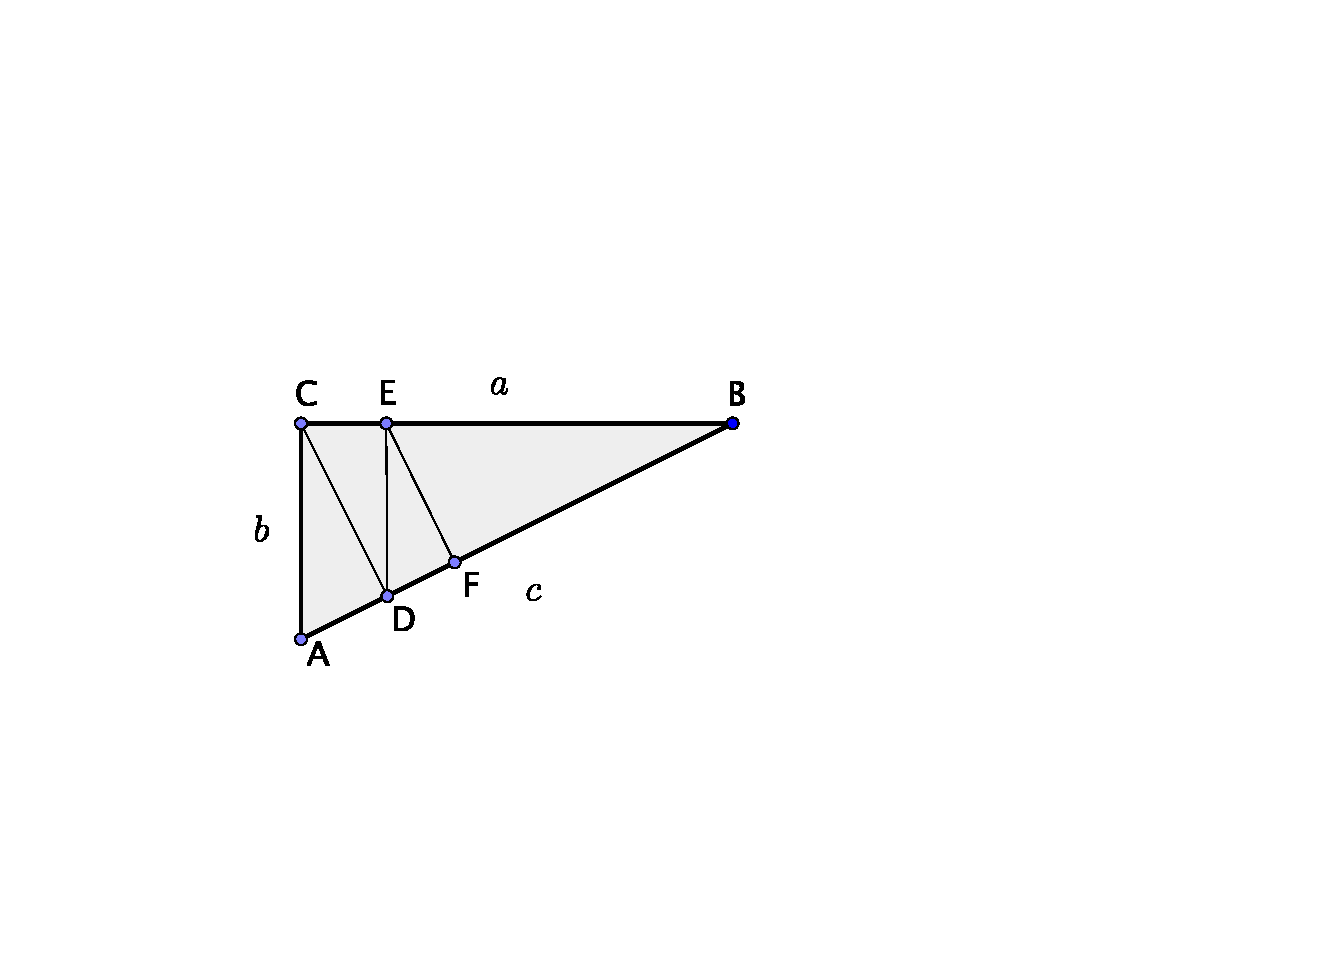
\includegraphics[width=0.38\textwidth]{img-09/fig17}
\end{center}
 
 \answers{Area ABC=1350; Area ACD=486; CD=36; DE=28.8; EF=23.04}
 
 \exer  Unint els punts mitjans dels costats d'un triangle s'obté un altre triangle. Com són? Quina relació hi ha entre els seus perímetres? I entre les seves àrees?
 
 \begin{center}
 	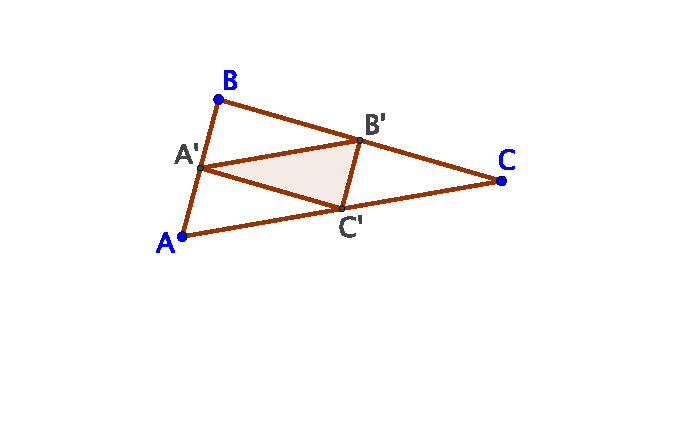
\includegraphics[width=0.38\textwidth]{img-09/fig20}
 \end{center}

\answers{Són semblants. El perímetre és la meitat i l'àrea la quarta part.}

\exer  Demostra que en dos triangles semblants les medianes són proporcionals. 

\answers{Si els costats són proporcionals, necessàriament les medianes també.}

\exer  Un triangle rectangle isòsceles té un catet de longitud 7 cm, igual a la hipotenusa d'un altre triangle semblant al primer. Quant valen les àrees de tots dos triangles?

\answers{24.5 cm$^2$ i 12.25 cm$^2$}

\exer  El mapa a escala 1:3000000 d'un poble té un àrea de 2500 cm${}^{2}$, quant mesura la superfície vertadera d'aquest poble?

\answers{$2500 \text{ cm}{}^2 \cdot \frac{(3\cdot 10^6)^2 \text{ cm}{}^2}{1 \text{ cm}{}^2}\cdot \frac{1 \text{ km}{}^2}{10^{10} \text{ cm}{}^2} = 2.25 \cdot 10^6 \text{ km}^2$}

\exer  L'altura i la base d'un triangle rectangle mesuren respectivament 4 i 7 cm; i és semblant a un altre de base 26 cm. Calcula l'altura del nou triangle i les àrees de tots dos.

\answers{L'altura $\frac{104}{7}=14.86$ cm; Les àrees són: 14 cm$^2$ i 193.14 cm$^2$}

\item \simbolsearch Per determinar el radi del Sol realitzam el següent experiment. Dirigim l'aparell de la figura cap el Sol i mesuram la mida de la taca es forma sobre la pantalla. Sabent que la llargària de l'aparell és de 1 m i la mida de la taca és aproximadament 1 cm, troba el radi del Sol. Hauràs de menester la distància entre la Terra i el Sol \linebreak 1 u.a.=150\, 000\, 000 km. 
\begin{center}
	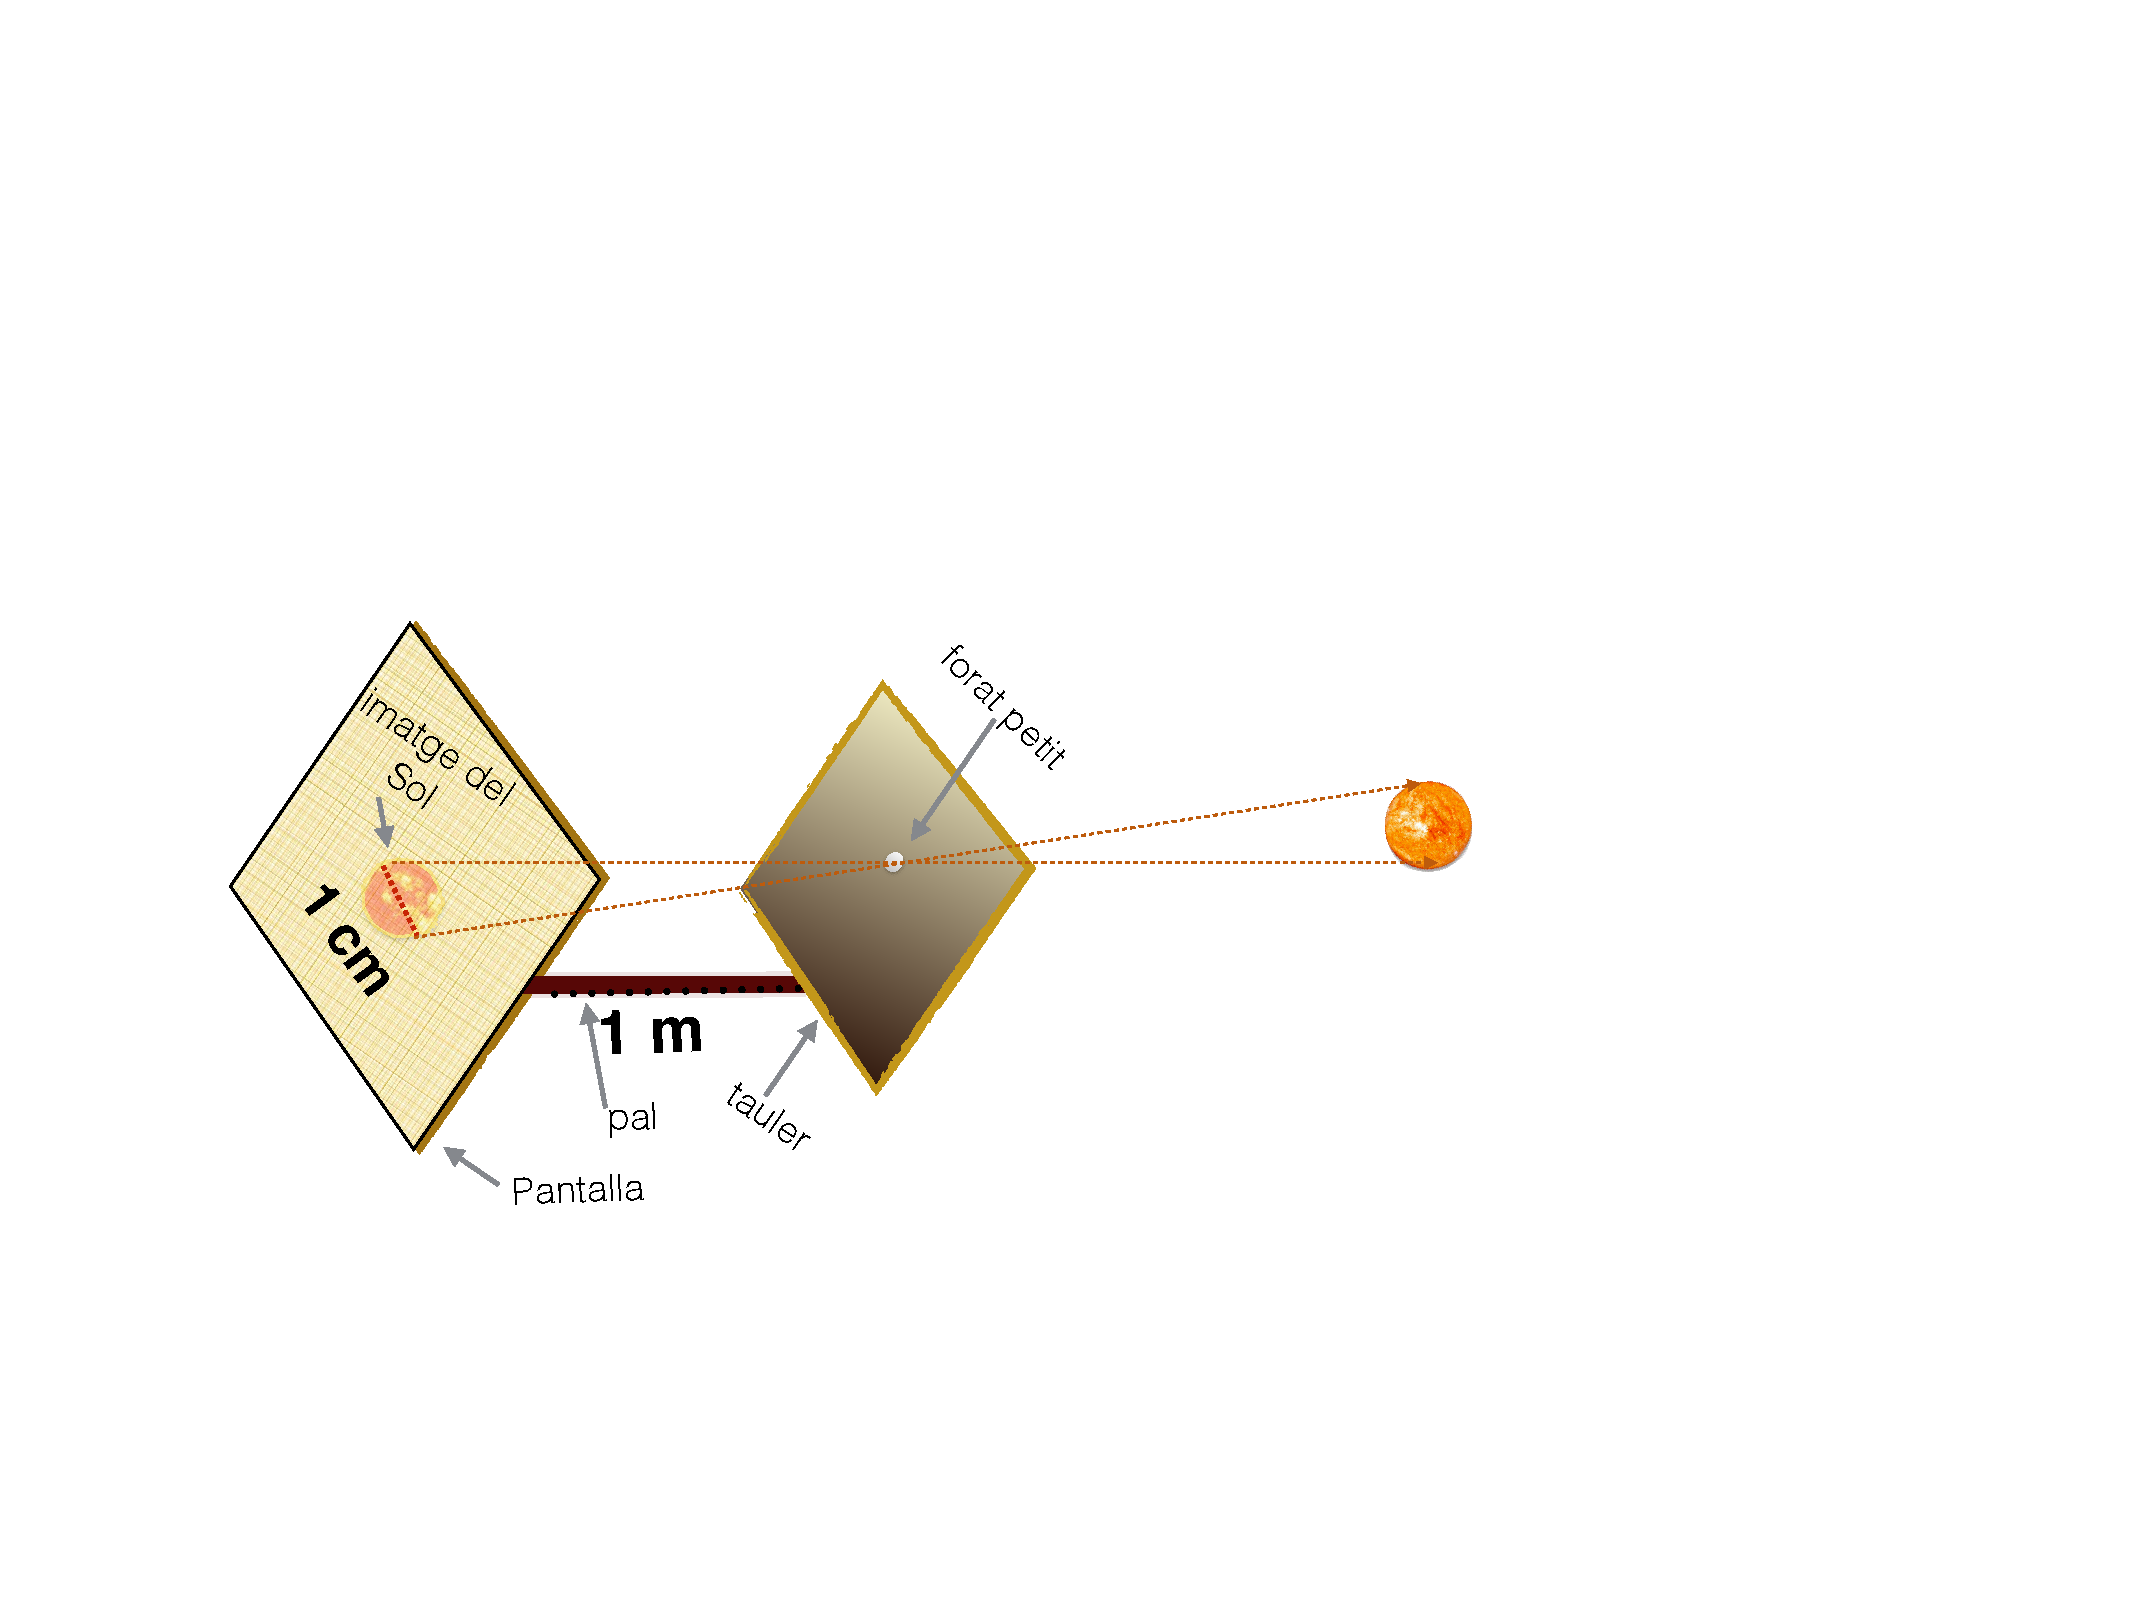
\includegraphics[width=6.7cm]{img-09/experiment-sol}
\end{center}
\end{mylist}
 
\answers{Per semblança $\frac{0.05}{R}=\frac{1}{1 500 000}$, $R=750 000$ km. El diàmetre del Sol és 1.5 milions de km.}
 


\subsection{Angles, longituds i àrees}

\begin{mylist} 
	
\exer Explica com es pot trobar el valor de l'angle desconegut $\alpha$ en cadascun dels casos següents:

\begin{center}
	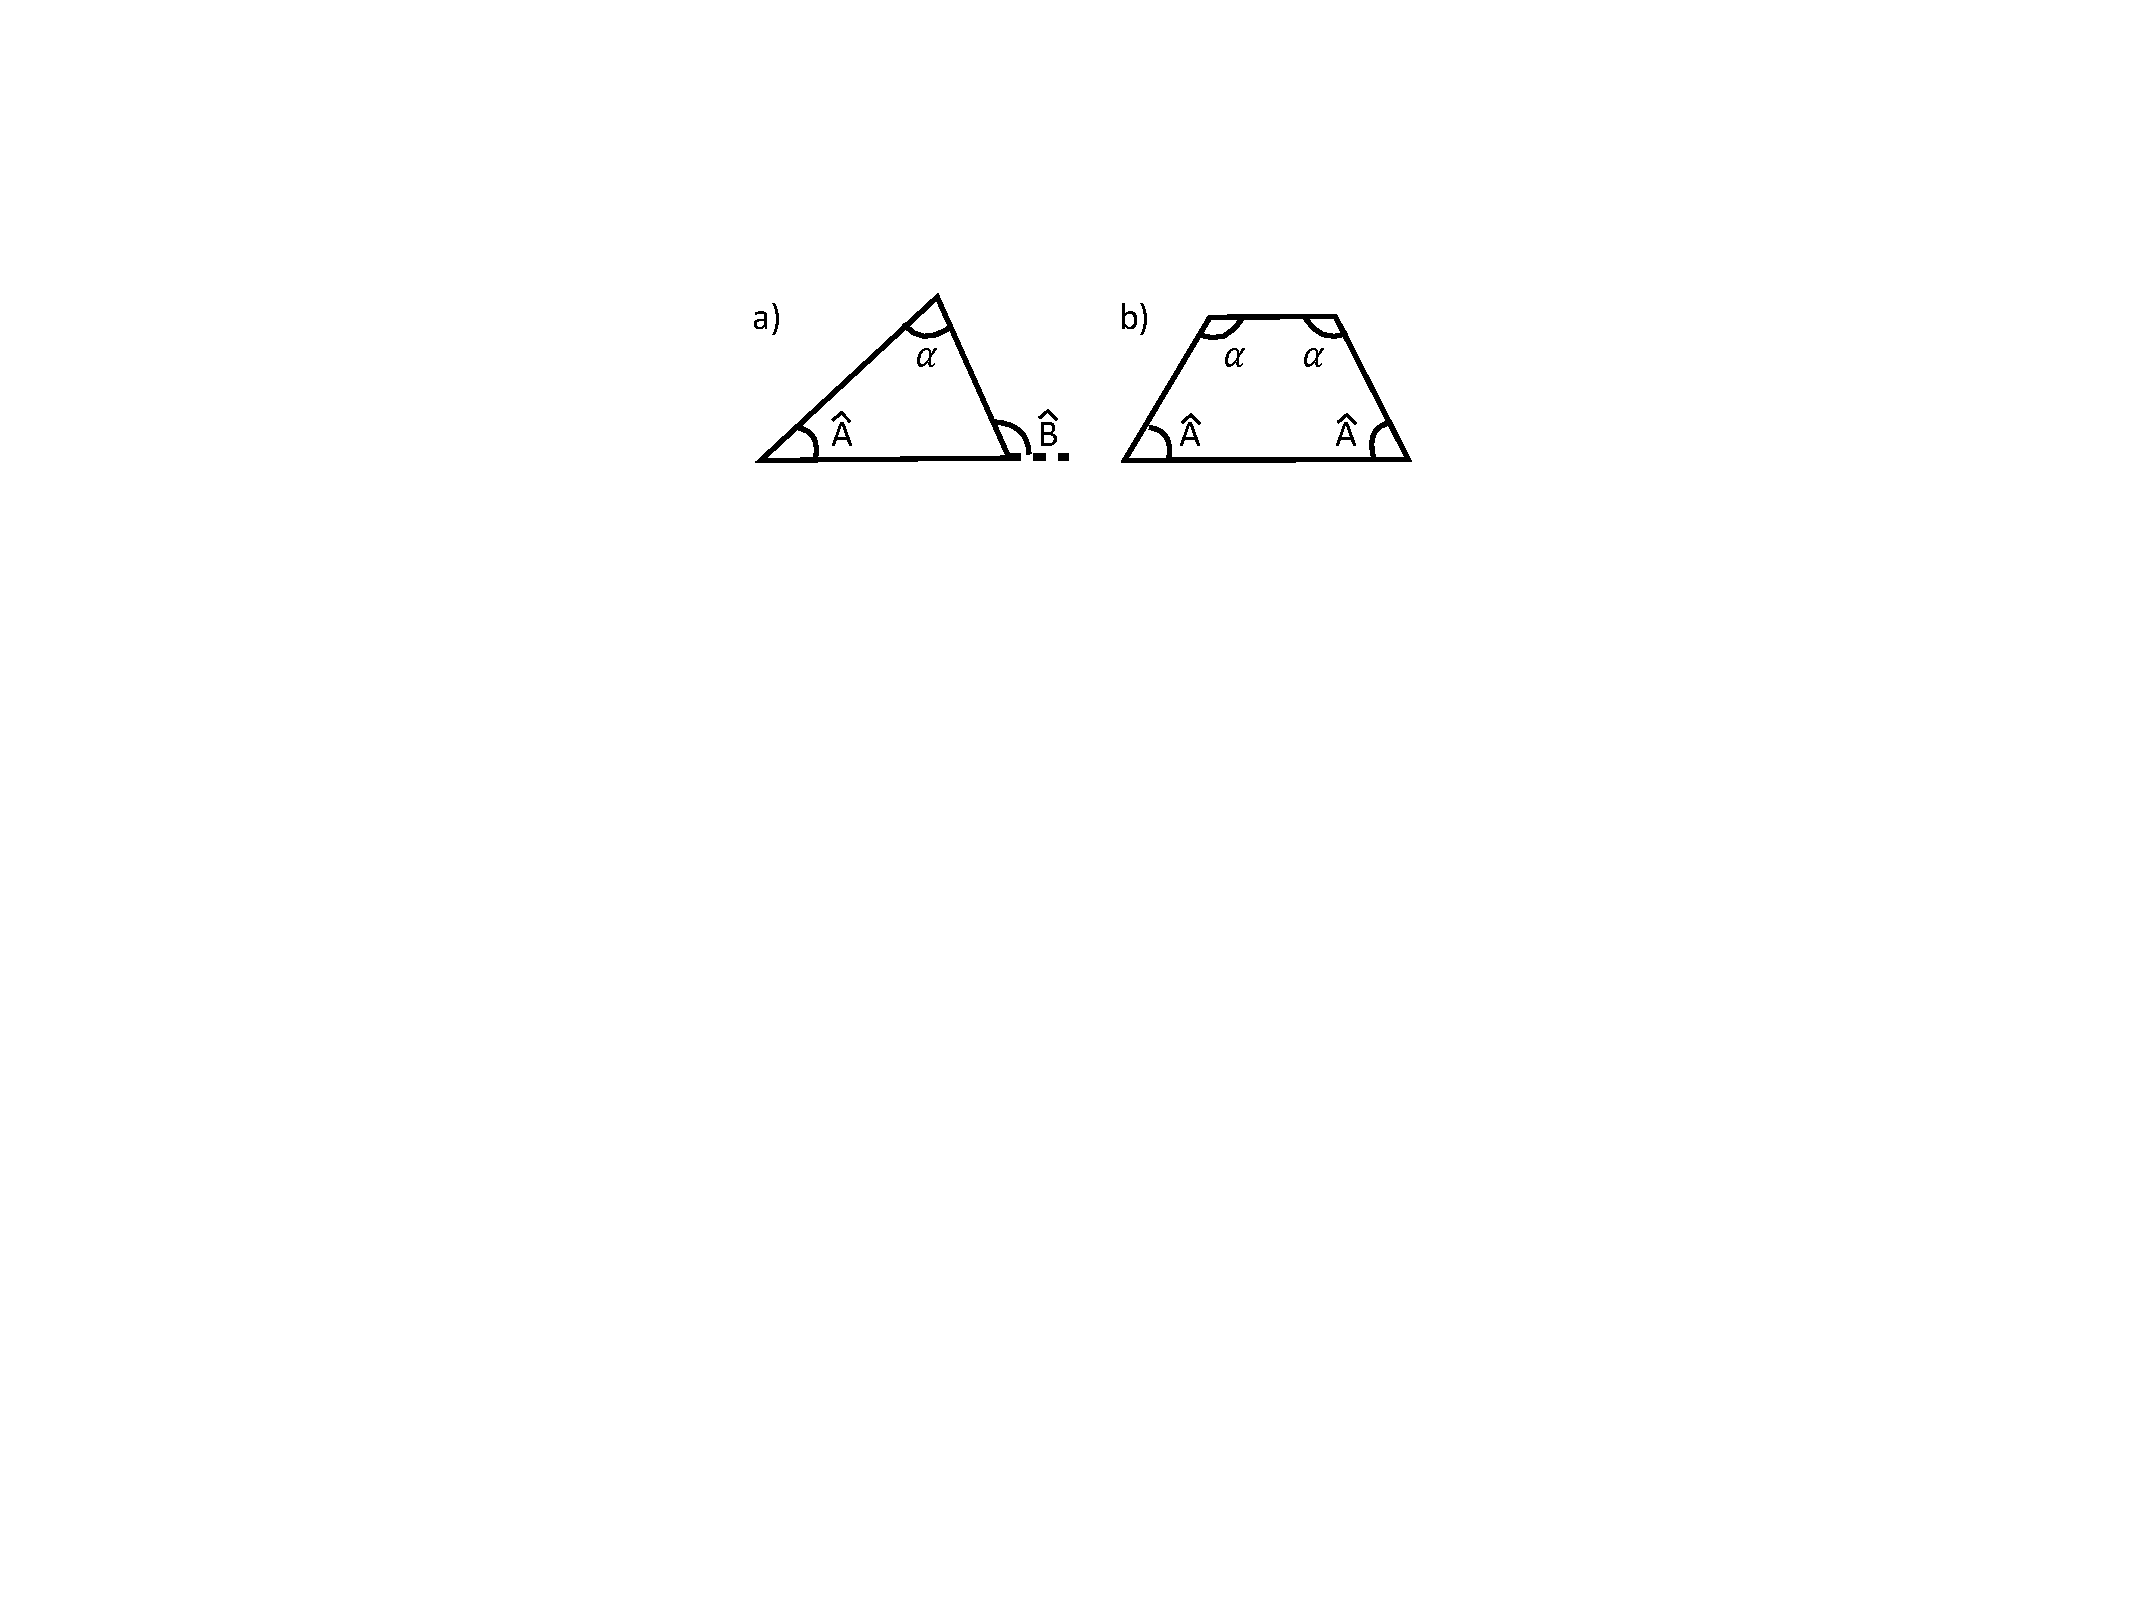
\includegraphics[width=0.4\textwidth]{img-09/angles}
\end{center}

\redacta

\answers{[$\alpha= 180 - (A+180-B)=B-A$, $2A+2\alpha=360$; $\alpha=180-A$]}

\exer  Calcula la longitud del costat d'un octògon regular inscrit en una circumferència de radi 5 cm.

\answers{El costat fa 3.8 cm}

\exer  Calcula l'apotema d'un hexàgon regular costat 7 cm.
\answers{$a_p=\frac{7}{2}\sqrt{3}=6.1$ cm}

\exer  Calcula l'àrea d'un cercle la circumferència del qual mesura 50 cm.
\answers{$A=\frac{25^2}{\pi}=198.94$ cm$^2$}

\exer  Calcula la longitud d'una circumferència el cercle de la qual té una superfície de mesura 50 cm${}^{2}$.
\answers{$L=10\sqrt{2\pi}=25.1$ cm$^2$}

\exer  La Terra fa una volta cada 24 hores, a quina velocitat es mou un punt sobre l'Equador?
\answers{L'equador fa 40000 km; La velocitat $v=50 000/3$ km/h}

\exer \hot Quina relació hi ha entre les àrees un triangle inscrit en un cercle i la del cercle?
\answers{Si el triangle és equilàter $\frac{3\sqrt{3}}{4\pi}$; sinó falten dades.}

\begin{comment}
\exer  Els grecs coneixien les dos següents possibles formes de construir un triangle rectangle amb els seus tres costats de longitud un nombre natural, sense més que donar valors a n. Comprova si es verifiquen per a n = 1, 2, {\dots}. 


\begin{tasks}
	\task  Catets: 2\textit{n} i \textit{n}${}^{2}$ -- 1, hipotenusa: \par \textit{n}${}^{2}$ + 1.  
	\task  Catets: 2\textit{n} + 1 i 2\textit{n}${}^{2}$ + 2\textit{n}, hipotenusa: 2\textit{n}${}^{2}$ + 2\textit{n} + 1.
\end{tasks}
\end{comment}

\exer  En augmentar en 3 cm el costat d'un quadrat la seva àrea augmenta 32 cm${}^{2}$. Quant mesura el costat de aquests quadrats?
\answers{$c=23/6$}

\exer  Es vol cobrir un terreny circular de 25 m de diàmetre amb graveta, tirant 10 kg per cada metre quadrat. Quanta graveta es necessita?
\answers{Necessita $4908.74$ kg. Aprox. 5 tones.}

\exer  Una escala de 4 m de longitud està recolzada sobre una paret. El peu de l'escala dista 1,5 m de la paret. Quina altura aconsegueix l'escala sobre la paret?
\answers{Arriba a una altura de 3.71 m}

\exer  Calcula l'àrea de la circumferència circumscrita a un rectangle de costats 7 i 9 cm.
\answers{$A=102.1$ cm$^2$}

\exer  Calcula l'àrea d'un hexàgon regular de 3 cm de costat. Allarga els costats de l'hexàgon i dibuixa un hexàgon estrellat. Calcula la seva àrea.
\answers{Hexàgon: 23.38 cm$^2$; Hexàgon estrellat: 46.77 cm$^2$}

\vspace{-1.5cm}
\exer \begin{minipage}[t]{0.3\textwidth}
	 El senyal de tràfic de STOP té forma d'octògon regular. La seva altura mesura 90 cm, i el seu costat 37 cm, quant mesura la seva superfície?
\end{minipage}
\begin{minipage}{0.15\textwidth}
	\centering
	\vspace{1.5cm}
	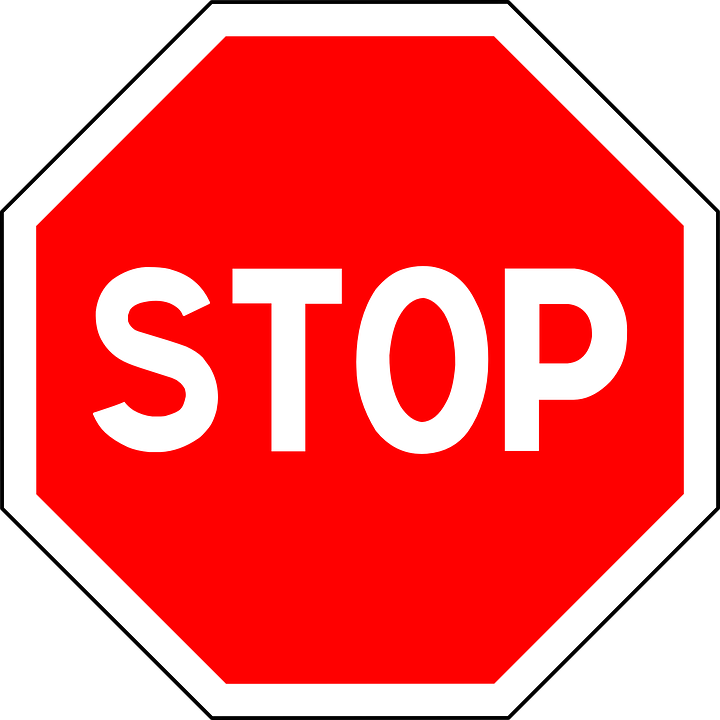
\includegraphics[width=0.75\textwidth]{img-09/stop}
\end{minipage}
\answers{Aprox. 6600 cm$^2$}

\exer \hot Calcula l'altura del trapezi de la figura. Després calcula'n l'àrea.

\begin{center}
	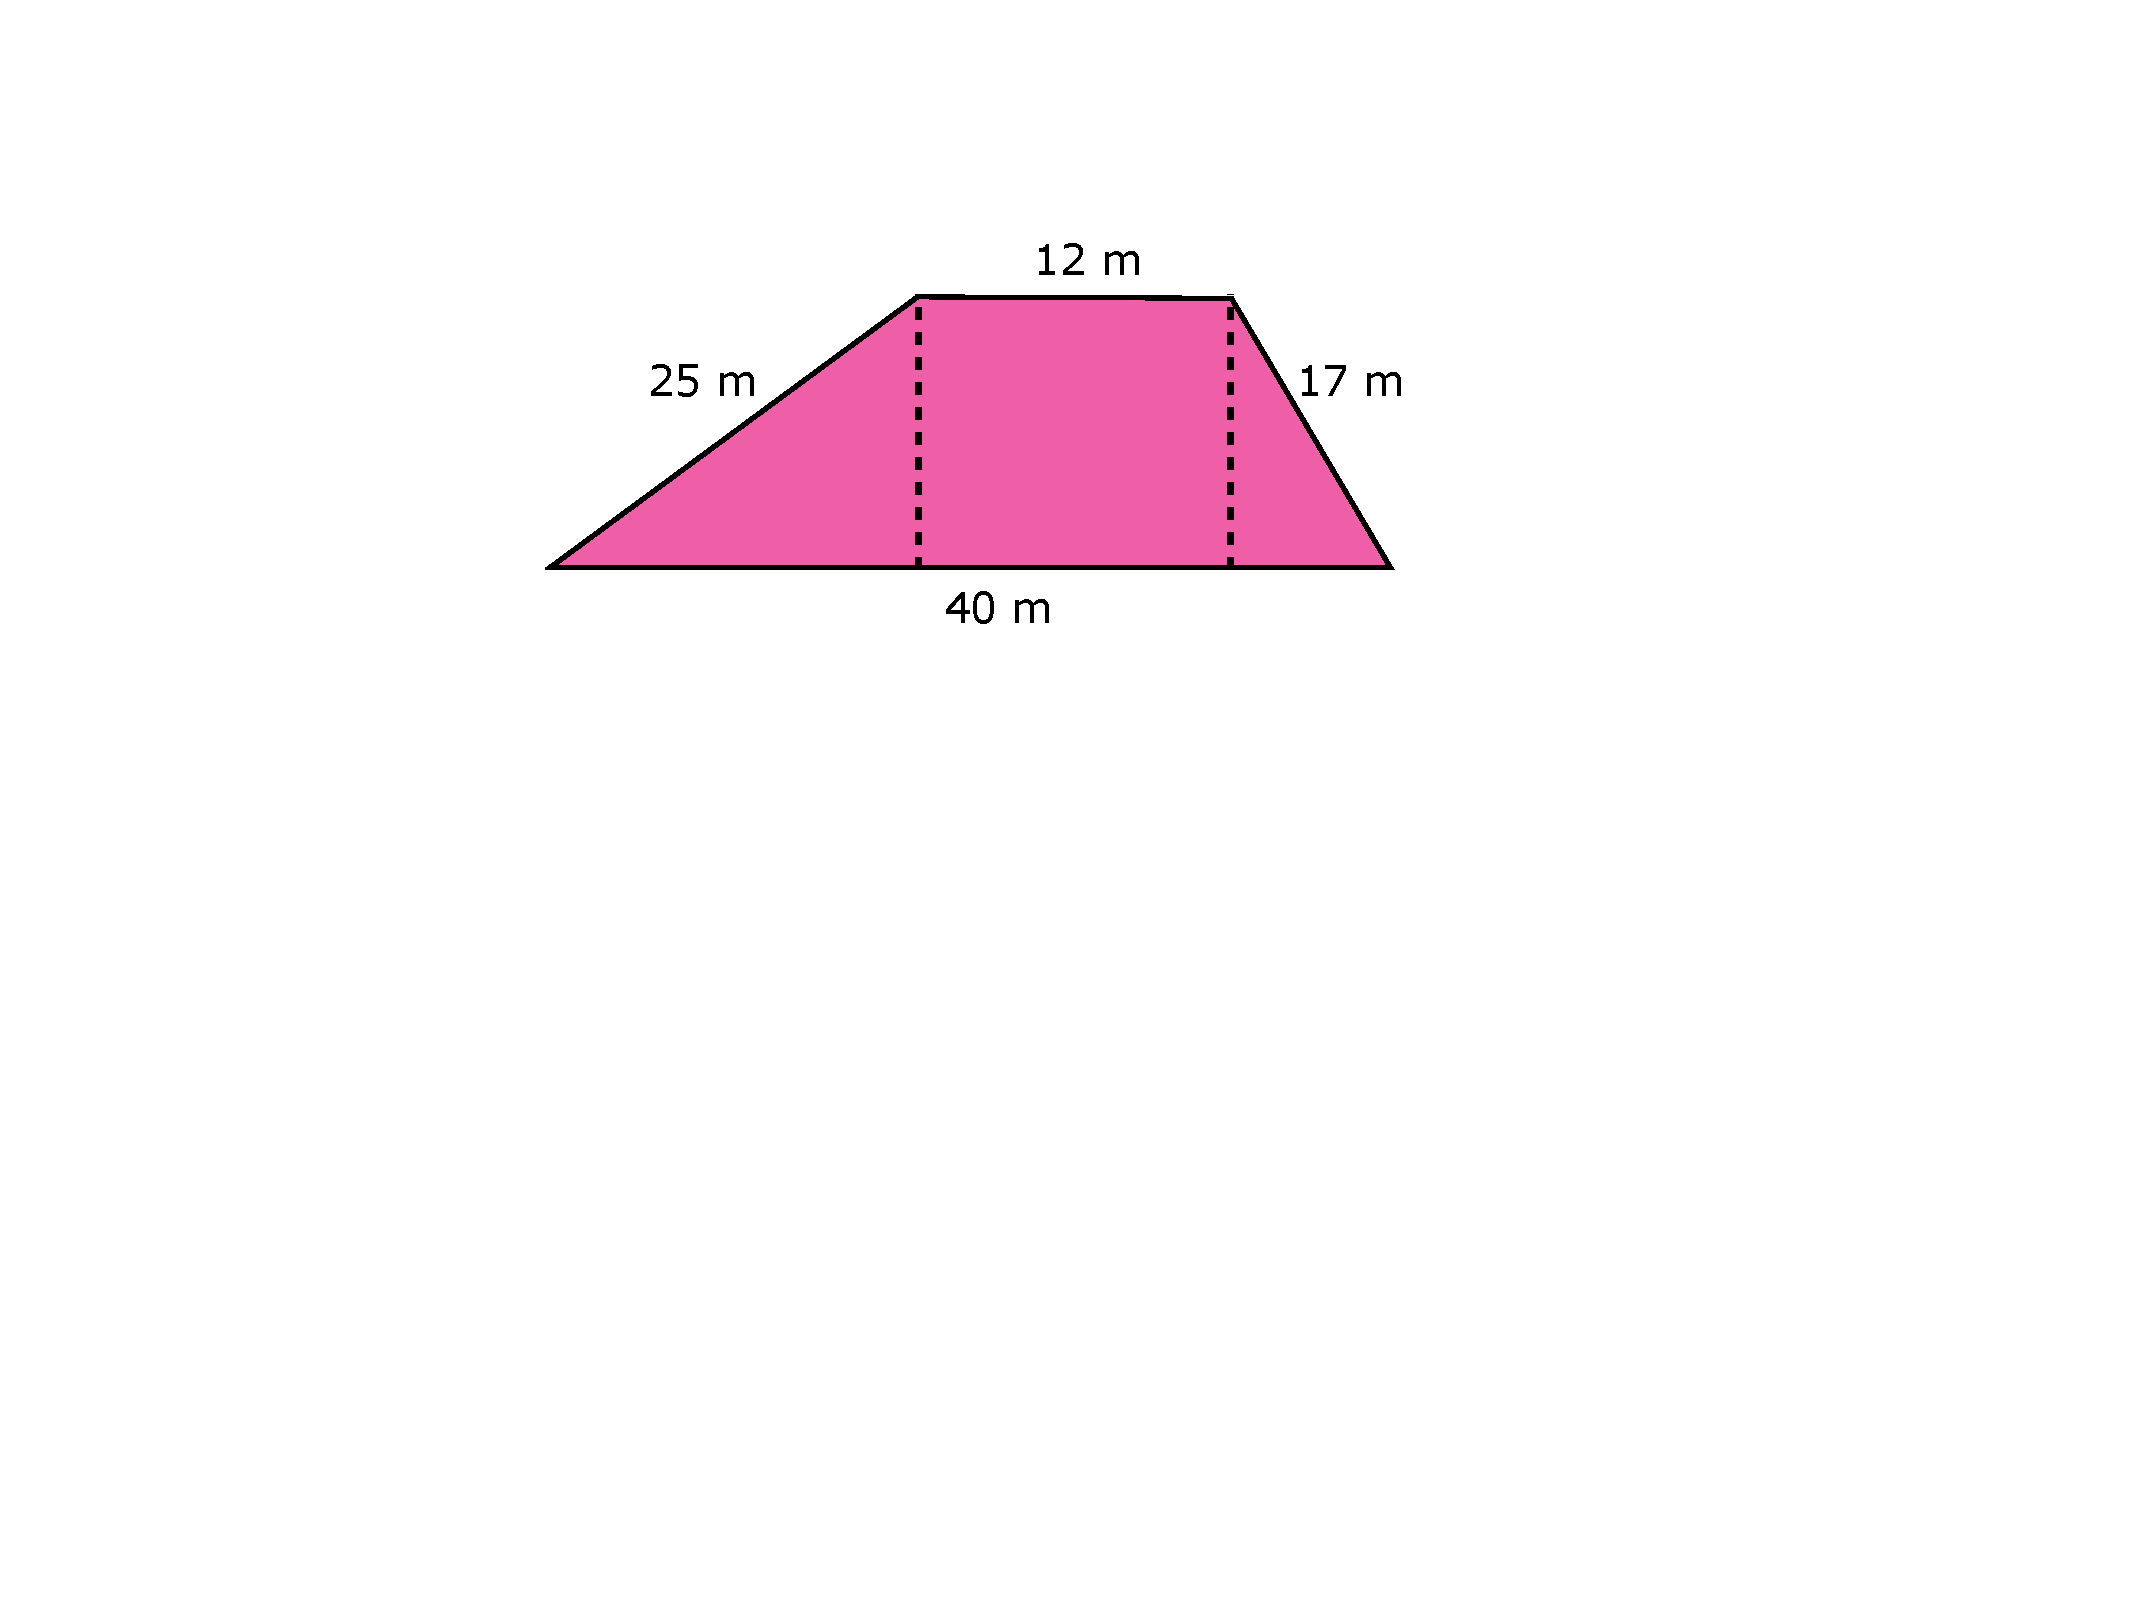
\includegraphics[width=6cm]{img-09/trapezi-exer}
\end{center}
\answers{$\left. \begin{array}{l} 25^2=x^2+h^2 \\ 17^2 =(28-x)^2+h^2 \end{array} \right\}$ \par
$x=20$ m i $h=15$ m.  L'àrea és $A=390$  m$^2$.}

\exer  Calcula l'àrea d'un triangle equilàter de costat 10 cm.
\answers{43.30 cm$^2$}

\exer  Calcula l'àrea d'un hexàgon regular de perímetre 60 cm.
\answers{259.81 cm$^2$}

\exer  Calcula l'àrea d'un trapezi isòsceles de base menor 5 cm, costat 3 cm i altura 4 cm.
\answers{Aquesta figura és impossible ja que l'altura 4 és major que el costat 3. Queda un triangle rectangle on la hipotenusa mesuraria menys que un catet.}

\exer  Calcula l'àrea d'un trapezi isòsceles de bases 8 i 6 cm i costat 3 cm.
\answers{$A=19.80$ cm$^2$}

\exer  Calcula l'àrea i el perímetre d'un rectangle de costat 4 cm i diagonal 7 cm.
\answers{$A=29.98$ cm$^2$ i $P=19.49$ cm}

\exer  Calcula l'àrea i el perímetre d'un quadrat de diagonal 9 cm.
\answers{$A=40.5$ cm$^2$ i $P=25.46$ cm}

\exer  Calcula l'àrea i el perímetre d'un triangle isòsceles de base 8 cm i altura 6 cm.
\answers{$A=24$ cm$^2$ i $P=22.42$ cm}

\exer  Un triangle mesura d'altura $\pi$ i de base $\pi$ + 1. És rectangle?
\answers{Estrictament no. Si suposam que $\pi=3$ i que la base i l'altura són els catets, llavors sí.}

\exer  Dibuixa un triangle rectangle isòsceles de catets de longitud 1, quant mesura la hipotenusa? Prenent aquesta hipotenusa com a catet i amb l'altre catet igual a 1 dibuixa un nou triangle rectangle. Quant mesura la nova hipotenusa? Continua el procés 4 vegades, quant mesura l'última hipotenusa?
\answers{$\sqrt{2}$, $\sqrt{3}$, $\sqrt{4}=2$, $\sqrt{5}$, $\sqrt{6}$}

\exer  Dibuixa un triangle rectangle de catets de longitud 1 i 2 cm, quant mesura la hipotenusa? Prenent aquesta hipotenusa com a catet i amb l'altre catet de longitud 1 cm dibuixa un nou triangle rectangle. Quant mesura la nova hipotenusa? Continua el procés 3 vegades, quant mesura la darrera hipotenusa?
\answers{$\sqrt{5}$, $\sqrt{6}$ i $\sqrt{7}$ cm}

\exer  Calcula l'altura d'una piràmide regular quadrangular de costat de la base 10 m i d'aresta 15 m.
\answers{$H=5\sqrt{7}=13.23$ cm$^2$}

\exer  Calcula la generatriu d'un con de radi de la base 5 m i d'altura 7 m.
\answers{$g=\sqrt{74}=8.602$ m}

\exer  Dos ascetes hindús viuen a la part alta d'un penya-segat de 10 m d'altura el peu del qual està a 200 metres del poble més proper. Un dels ascetes baixa del penya-segat i va al poble. L'altre, que és mag, ascendeix una distancia $x$ i viatja volant en línia recta al poble. Tots dos recorren la mateixa distància. Quant ha ascendit el mag?
\answers{$-10+10\sqrt{41}=54.03$ m}

\exer  Quant mesura l'aresta de la base de la piràmide de Kheops si mesura 138 m d'altura i 227 m d'aresta?
\begin{center}
	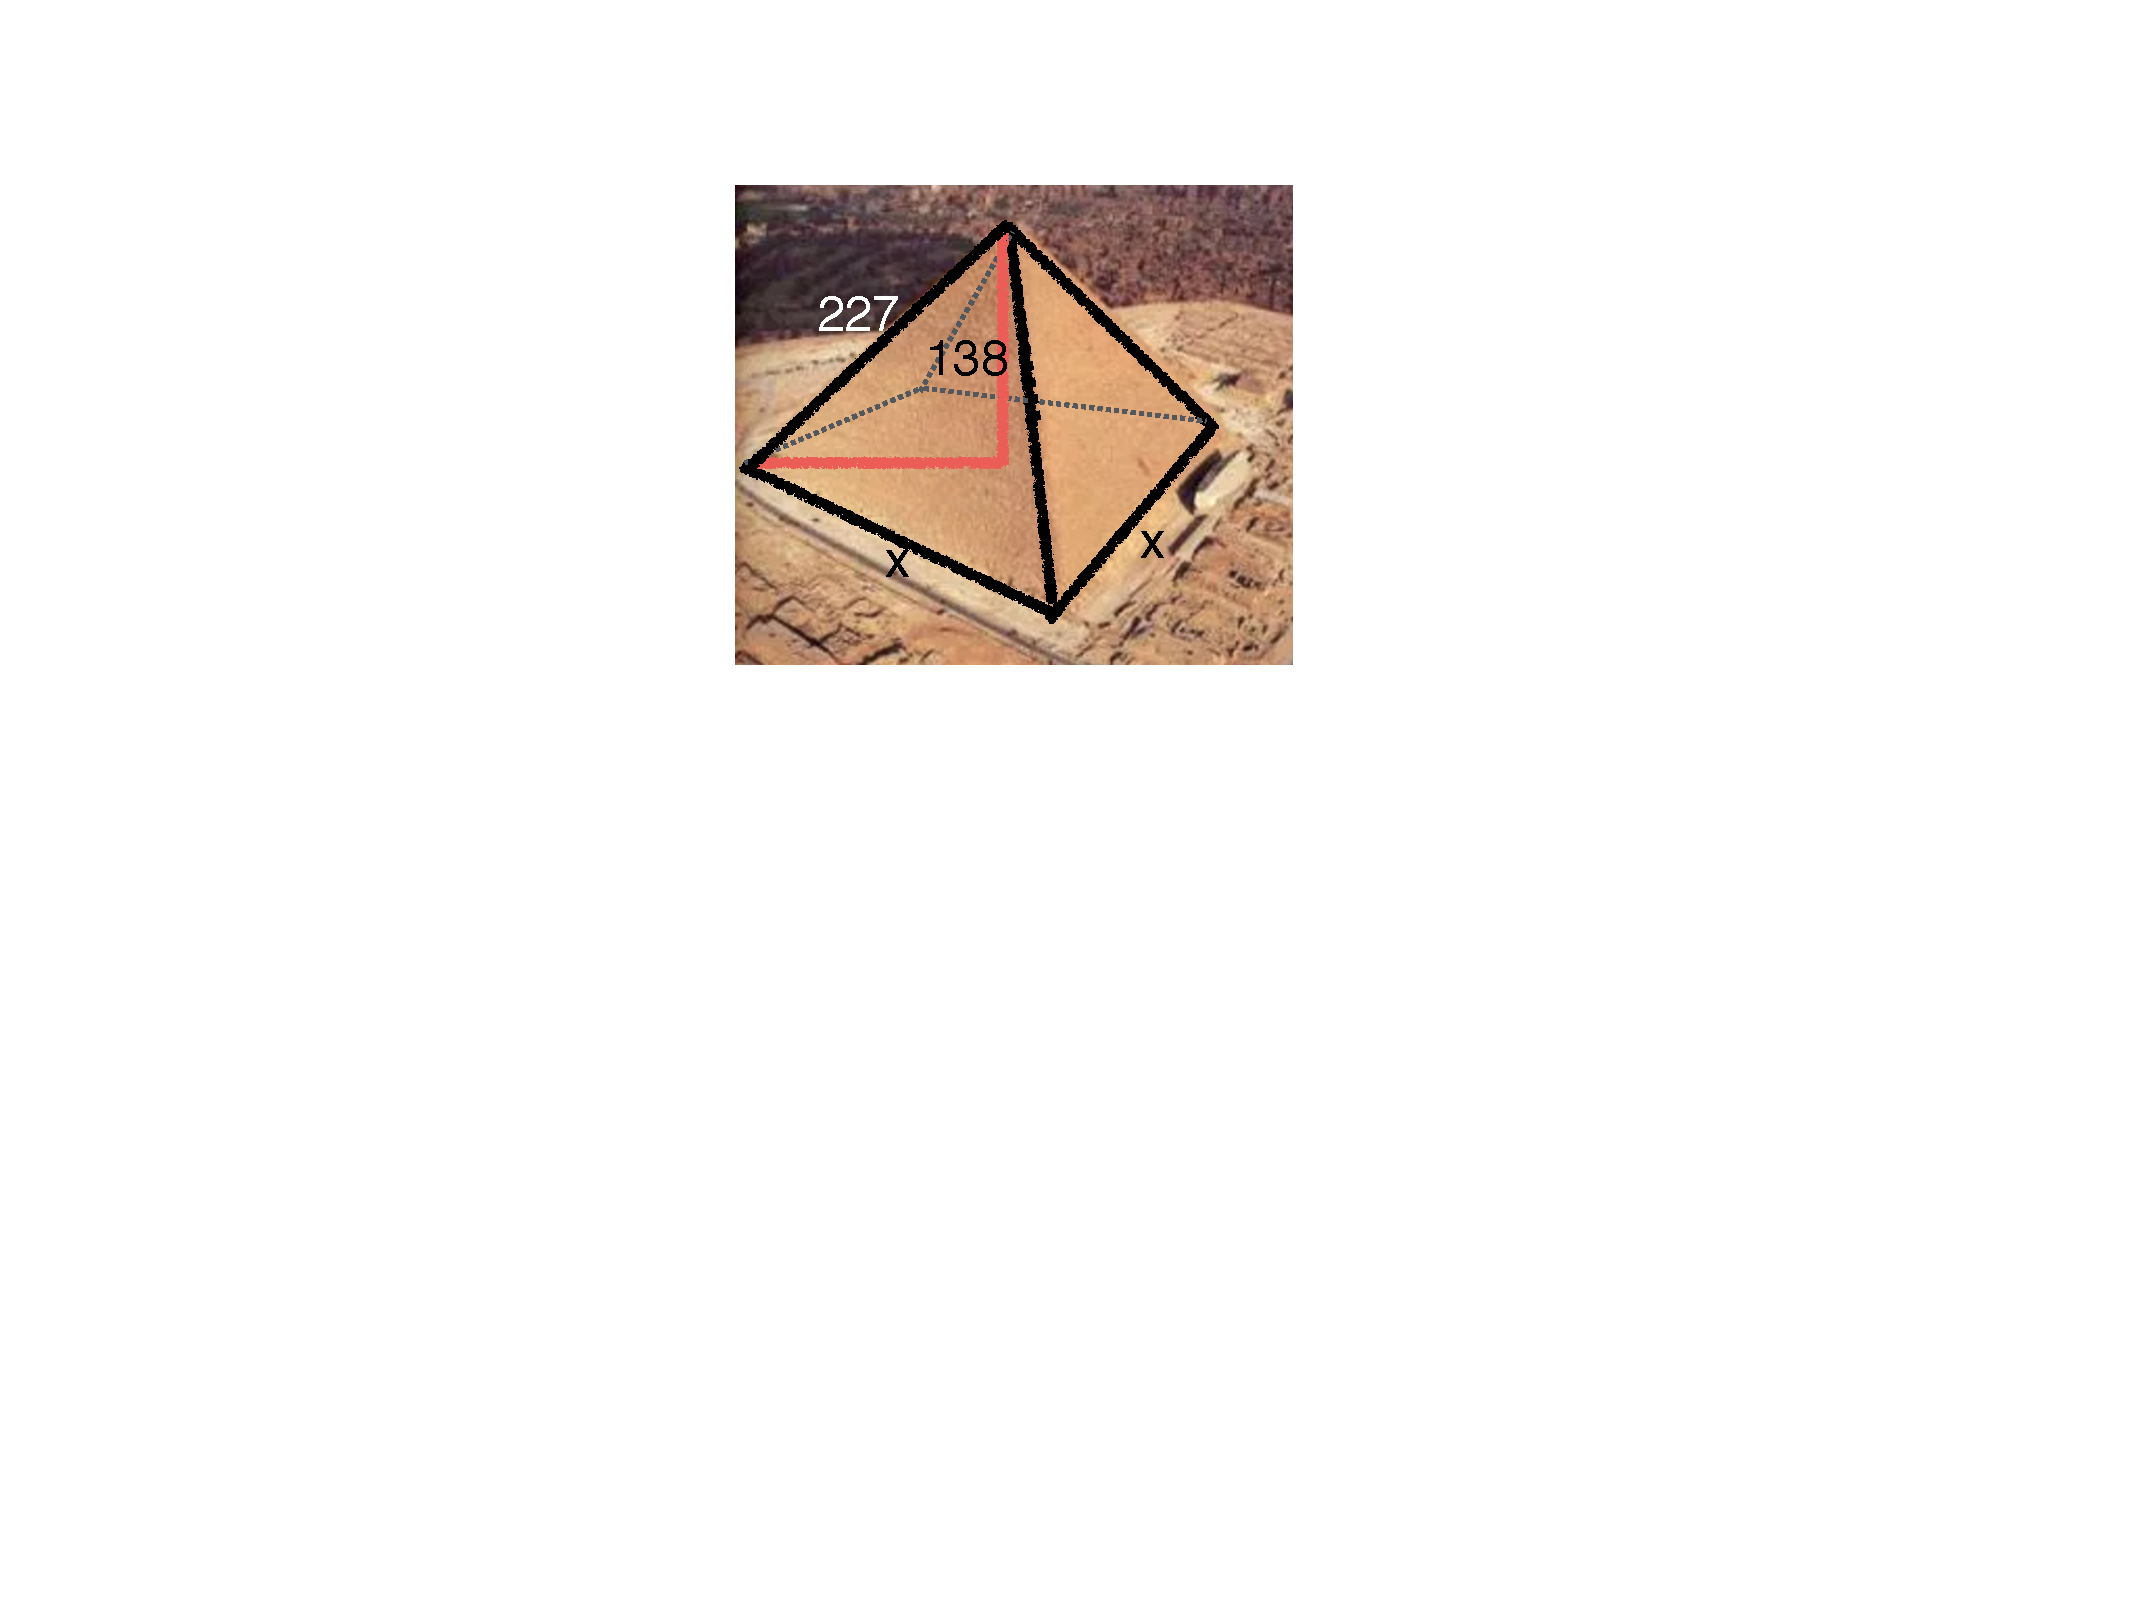
\includegraphics[width=0.3\textwidth]{img-09/keops}
\end{center}
\answers{$x=211.681$}

\end{mylist}


\subsection{Llocs geomètrics}

\begin{mylist}
	\exer  Dibuixa en el teu quadern un triangle de costats 2 cm, 3 cm i 4 cm. Traça en ell, utilitzant regla i compàs, les mediatrius i bisectrius. Determina el circumcentre i l'incentre. Traça les circumferències inscrites i circumscrites.
	
	\exer  Dibuixa en el teu quadern un triangle de costat 5 cm i angles adjacents al mateix de 30${}^\circ$  i 50${}^\circ$ . Traça en ell, utilitzant regla i compàs, les medianes i les altures. Determina el seu ortocentre i el seu baricentre.
	
	\exer  Dibuixa en el teu quadern un triangle amb un angle de 50${}^\circ$  comprès entre dos costats de 5 i 8 cm. Obté el seu circumcentre i el seu incentre.
	
	\exer  Com són les rectes i punts notables d'un triangle rectangle?
	
	\exer  Com són les rectes i punts notables d'un triangle isòsceles?


\end{mylist}
\end{activitats}

\pagebreak
\begin{autoaval}{50}
\begin{mylist}
\exer[2]  Tots els punts que estan a la mateixa distància de dos punts donats estan en:

\begin{tasks}(4)
	\task  una bisectriu   
	\task  una circumferència   
	\task  una el·lipse   
	\task  una mediatriu 
\end{tasks}
\answers{\textbf{--10.} Autoavaluació: 1d; 2b; 3c; 4a; 5d; 6a; 7a; 8c; 9d; 10a}

\exer  Les tres medianes d'un triangle es tallen en el:

\begin{tasks}(4)
	\task  ortocentre   
	\task  baricentre   
	\task  incentre   
	\task  circumcentre 
\end{tasks}


\exer  El circumcentre és el centre de:

\begin{tasks}(2)
	\task  gravetat del triangle  
	\task  la circumferència inscrita   
	\task  la circumferència  circumscrita 
\end{tasks}


\exer  Dos triangles són semblants si:

\begin{tasks}(2)
	\task  tenen dos angles iguals    
	\task  tenen dos costats proporcionals
	\task  tenen un angle igual    
	\task  les seves àrees són semblants
\end{tasks}


\exer  Sabem que els triangles \textit{ABC} i \textit{A'B'C'} són semblants. Calcula el valor de a'  i \textit{c'} perquè el siguin, sabent que \textit{a =} 10 cm, \textit{b} = 6 cm, \textit{b'} = 3 cm, \textit{c} = 8 cm: 

\begin{tasks}(2)
	\task  \textit{a '} = 4 cm i \textit{c'} = 6 cm    
	\task  \textit{a'} = 5 cm i \textit{c'} = 6 cm 
	\task  \textit{a'} = 4 cm i \textit{c'} = 4 cm    
	\task  \textit{a'} = 5 cm i \textit{c'} = 4 cm
\end{tasks}


\exer  Si la hipotenusa d'un triangle rectangle mesura 7 cm i un catet mesura 3 cm, llavors l'altre catet mesura aproximadament:

\begin{tasks}(4)
	\task  6,3 cm    
	\task  5 cm    
	\task  5,8 cm   
	\task  6,9 cm
\end{tasks}


\exer  La suma dels angles interiors d'un polígon irregular de deu costats val:

\begin{tasks}(4)
	\task  1440${}^\circ$     
	\task  1620${}^\circ$     
	\task  1800${}^\circ$    
	\task  1260${}^\circ$ 
\end{tasks}


\exer  L'àrea d'un rombe de costat 5 cm i una diagonal de 8 cm mesura:

\begin{tasks}(4)
	\task  48 cm${}^{2}$  
	\task  36,7 cm${}^{2}$  
	\task  24 cm${}^{2}$   
	\task  21,2 cm${}^{2}$
\end{tasks}

 


\exer  L'angle central de l'inscrit en la circumferència que abasta un angle de 72${}^\circ$  mesura: 

\begin{tasks}(4)
	\task  720${}^\circ$     
	\task  108${}^\circ$      
	\task  36${}^\circ$     
	\task  144${}^\circ$ 
\end{tasks}


\exer  La longitud de la circumferència i l'àrea del cercle de radi 3 cm són respectivament:

\begin{tasks}(4)
	\task  6$\pi$ cm i 9$\pi$ cm${}^{2}$ 
	\task  9$\pi$ cm i 6$\pi$ cm${}^{2}$  
	\task  3$\pi$ cm i 3$\pi$ cm${}^{2}$  


	\task  18 cm i 27 cm${}^{2}$
\end{tasks}

\end{mylist}

\end{autoaval} 


\newpage
\resum \label{sec:resumarees}
\begin{center}
	\renewcommand{\arraystretch}{1.6}
	\begin{tabular}{|P{0.46\textwidth}|p{0.46\textwidth}|} \hline
		\rowcolor{lightgray} \textbf{Triangle} &   \textbf{Quadrat} \\ \hline
			\begin{tabular}{m{0.25\textwidth}m{0.2\textwidth}}
			\begin{center} 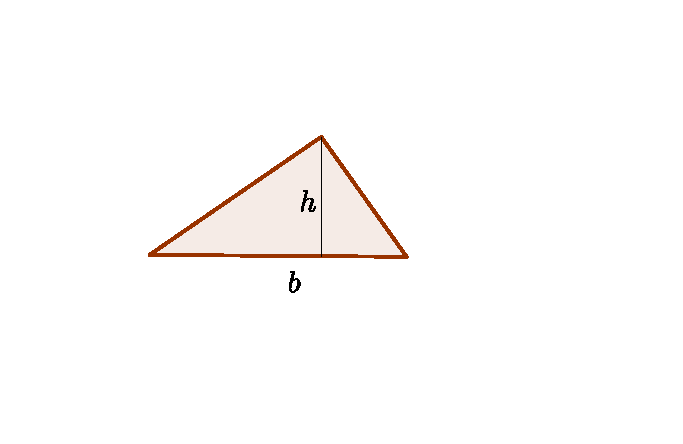
\includegraphics[width=0.25\textwidth]{img-09/triangle} \end{center} &  \begin{center} 	$Area = \frac{b\cdot h}{2}$   \end{center}
		\end{tabular}
		& 
		\begin{tabular}{m{0.25\textwidth} m{0.2\textwidth}}
			\centering 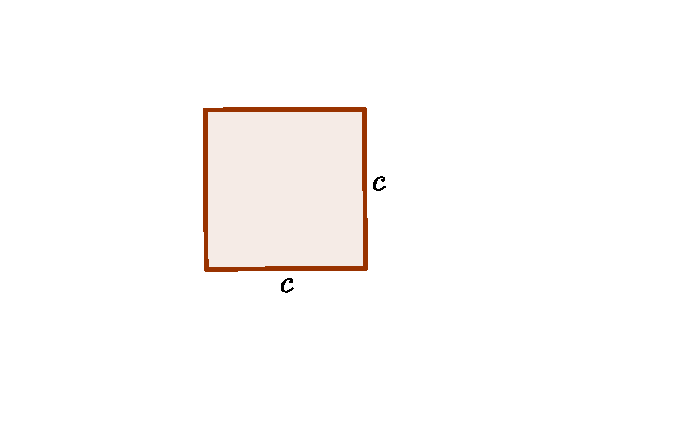
\includegraphics[width=0.25\textwidth]{img-09/quadrat} &   \begin{center} $Area = c^2$ \end{center}
		\end{tabular}
		\\ \hline
		
		
			\rowcolor{lightgray} \textbf{Rectangle} &   \textbf{Paral·lelogram} \\ \hline
		\begin{tabular}{m{0.25\textwidth}m{0.2\textwidth}}
			\begin{center} 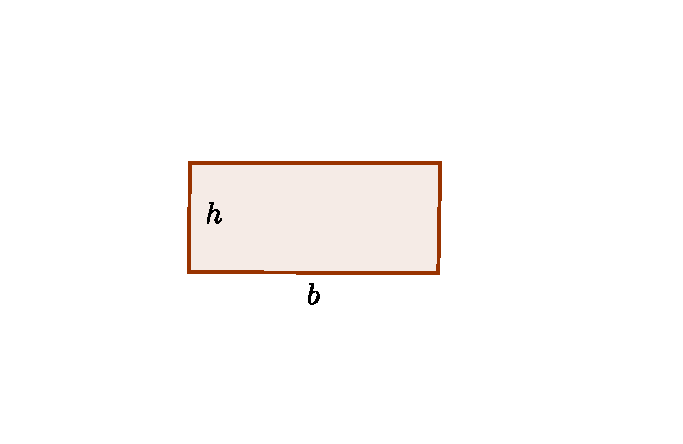
\includegraphics[width=0.25\textwidth]{img-09/rectangle} \end{center} &  \begin{center} 	$Area =b \cdot h$   \end{center}
		\end{tabular}
		& 
		\begin{tabular}{m{0.25\textwidth} m{0.2\textwidth}}
			\centering 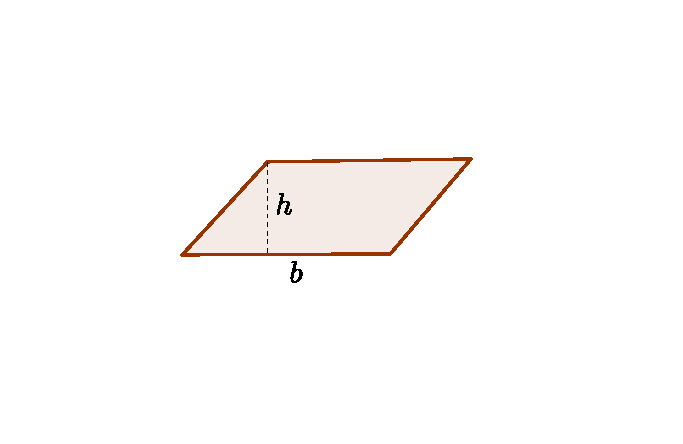
\includegraphics[width=0.25\textwidth]{img-09/parallelogram} &   \begin{center} $Area =b\cdot h$ \end{center}
		\end{tabular}
		\\ \hline
		
		
			\rowcolor{lightgray} \textbf{Rombe} &   \textbf{Trapezi} \\ \hline
		\begin{tabular}{m{0.25\textwidth}m{0.2\textwidth}}
			\begin{center} 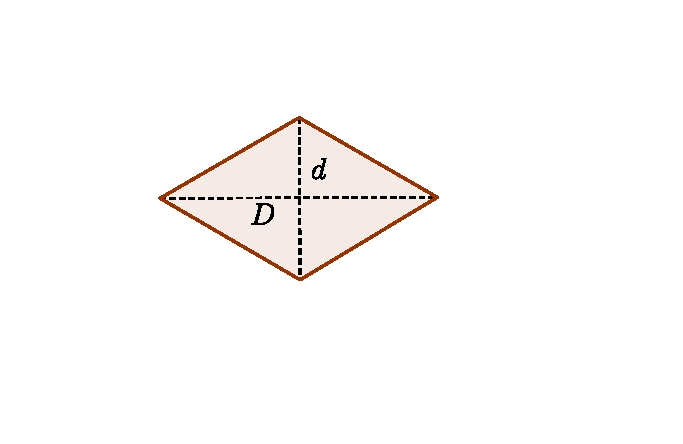
\includegraphics[width=0.25\textwidth]{img-09/rombe} \end{center} &  \begin{center} 	$Area = \frac{D\cdot d}{2}$   \end{center}
		\end{tabular}
		& 
		\begin{tabular}{m{0.21\textwidth} m{0.2\textwidth}}
			\centering 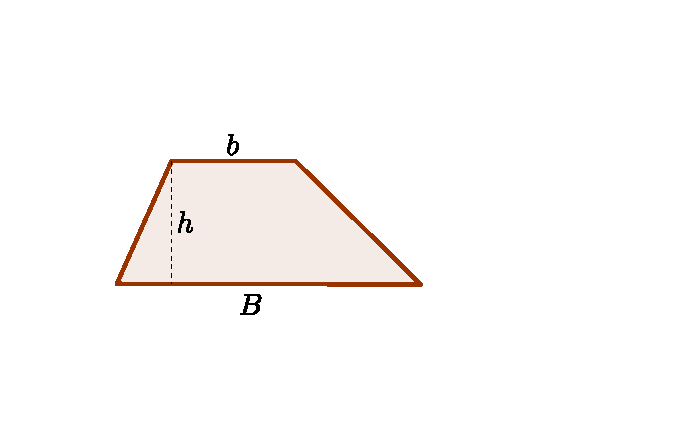
\includegraphics[width=0.22\textwidth]{img-09/trapezi} &   \begin{center} $Area = \frac{(B+b)\cdot h}{2}$ \end{center}
		\end{tabular}
		\\ \hline
		
			\rowcolor{lightgray} \textbf{Poligon regular} &   \textbf{Cercle} \\ \hline
		\begin{tabular}{m{0.2\textwidth}m{0.2\textwidth}}
			\begin{center} 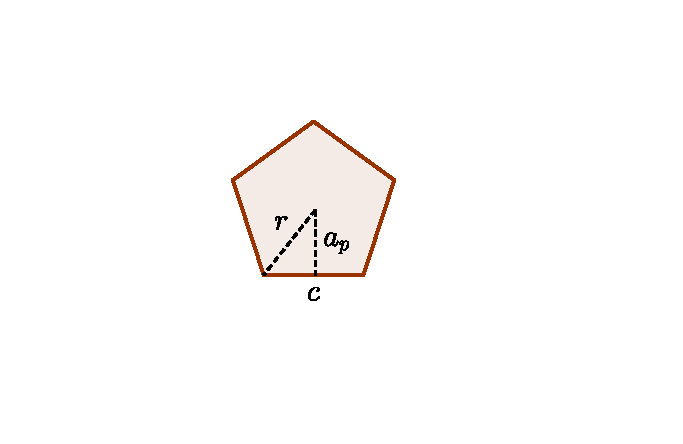
\includegraphics[width=0.23\textwidth]{img-09/poligon} \end{center} &  \begin{center} 	$Area = \frac{P\cdot a_p}{2}$ \par $P$: perímetre \par $a_p$: apotema   \end{center}
		\end{tabular}
		& 
		\begin{tabular}{m{0.2\textwidth} m{0.2\textwidth}}
			\centering 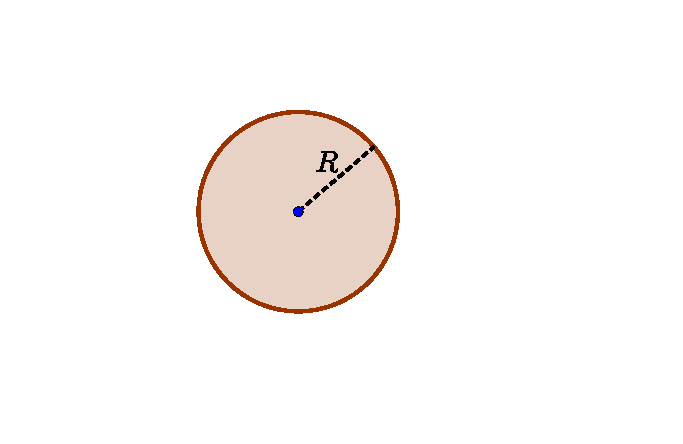
\includegraphics[width=0.2\textwidth]{img-09/cercle} &   \begin{center} $Area = \pi\, R^2$ \par $L=2\pi \, R$ \end{center}
		\end{tabular}
		\\ \hline
		
		
			\rowcolor{lightgray} \textbf{Sector circular} &   \textbf{Corona circular} \\ \hline
		\begin{tabular}{m{0.2\textwidth}m{0.2\textwidth}}
			\begin{center} 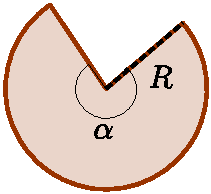
\includegraphics[width=0.2\textwidth]{img-09/sector} \end{center} &  \begin{center} 	$Area = \pi R^2 \frac{\alpha}{360}$ \par  $L = 2 \pi R \frac{\alpha}{360}$    \end{center}
		\end{tabular}
		& 
		\begin{tabular}{m{0.2\textwidth} m{0.2\textwidth}}
			\centering 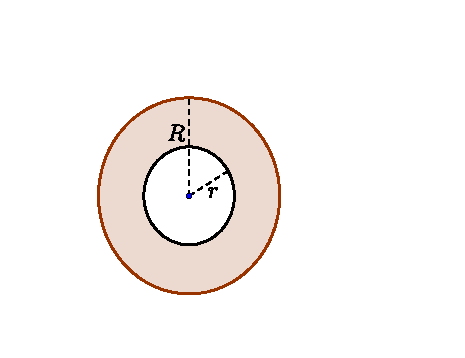
\includegraphics[width=0.2\textwidth]{img-09/corona} &   \begin{center} $Area = \pi (R^2-r^2)$ \end{center}
		\end{tabular}
		\\ \hline
	 
		  
	\end{tabular}
\end{center}